\documentclass[12px]{article}

\title{Metodi Numerici di Approssimazione - Appunti Completi}
\author{Federico De Sisti}
\date{\today}

\input{../../setup.tex}

\begin{document}
\maketitle
\tableofcontents
\newpage
\part{Lezione 1 Metodi Numerici di Approssimazione}
% --- Content from Lezione_01 ---
	\section{Introduzione}
	$y:(0,T)  \rightarrow\R^n$  è una curva detta variabile di stato\\
	$f:(0,T)\times \R^n \rightarrow \R^n$ è detta dinamica\\

	\textbf{Esempio:}\\
	$f = f(y) = y$ è il campo identità,  $y = (y_1,y_2)\in\R^2 \ \ f(y)\in \R^2$\\
	$\dot y = f(y) = y$\\
	 $\dot y_1 = y_1, \ \ \dot y_2 = y_2$\\
	 In questo caso molto semplice il sistema è disaccoppiato sulle componenti.\\
	 La soluzione è $e^t + c$\\
	 \[
	 y(0) = y_0 = (y_1^0, y_2^0)
	 .\] 
	 $ \Rightarrow  y_1(t) = y_1^0e^t$\\
	 $  y_2(t) = y_2^0e^t$\\
	 Il punto $(1,0)$ inizia a postarti verso destra con velocità che cresce esponenzialmente.\\
\textbf{Esempio:}\\
$f(y) = g(y_1,y_2)= (y_2,-y_1), \ \ \ f(1,0) = (0,-1), \ \ f(0,1) = (1,0)$\\
$|y| = \sqrt{y_1^2 + y_2^2}, \ \ |f(y)| = |(y_2-y_1)| = \sqrt{y_1^2 + y_2^2} = |y|$\\
In ogni punto la traiettoria di una particella introdotta nel campo deve essere tangente al campo.\\
Il moto sarà ciroclare uniforme, posso cercare soluzioni della forma
\[
\begin{cases}
	y_1(t) = A\cos t + B\sin t, \ \ \ \ y_1(0) = y_1^0\\ 
	y_2(t) = C\cos t + D\sin t, \ \ \ \ y_2(0) = y_2^0 
\end{cases}\ \ \ \ \ \ \text{ è una guess sulla soluzione}
.\] 
\[
\begin{cases}
	\dot y_1 = y_2\ \ \ \ \dot y_1 = -A\sin t + B\cos t = C\cos t + D\sin t\\
	\dot y_2 =- y_1 \ \ \ \ \dot y_2 = -C\sin t + D\cos t = -A\cos t - B\sin t
\end{cases}\circledast
.\]
Sto imponendo che la soluzione verifiche l'equazione.
\[
y_1(0) = y_1^0 = A, \ \ \ y_2(0) = y_2^0 = C
.\] 
\[
\begin{cases}
	B = C = y_2^0\\
	D = -A = -y_1^0
\end{cases} \text{che ricavo siccome }\circledast\text{ deve valere sempre}
.\] 
Quindi
\[
y_1(t) = y_1^0\cos t + y_2^0 \sin t
.\] 
\[
y_2(t) = y_2^0 - y_1^0\sin t
.\] 
Ad esempio per $y_0 = (1,0) \Rightarrow  Y(t) = (\cos t, - \sin t)$ è l'oscillatore armonico.\\
Un sistema dinamico è una relazione che coinvolge una curva e un campo di velocità.\\
In un sistema meccanico ci sono delle forze, cioè serve introdurre anche le accelerazioni.\\
\[
	F = ma \ \ \text{ Legge di Newton}
.\] 
$y$ è la posizione $y\in \R$\\
 $\dot y$ è la velocità  $\dot y\in \R$\\
  $\ddot y$ è l'accelerazione $\ddot y\in \R$\\
  si può quindi scrivere  $m\ddot y = F$ con  $F$ forza che dipende dal sistema. La più semplice è la forza elastica, possiamo scrivere
  \[
  m\ddot y = F = -ky
  .\] 
  che è lineare perché deriva da Taylor al primo ordine\\
  $\ddot y = -\frac k m y$\\
  Ogni sistema meccanico si può riscrivere come un sistema dinamico aumentando il numero di variabili. Pongo $\dot y = v$ E allora
   \[
	   \ddot y = \dot v = -\frac k my
  .\] 
  Quindi nella coppia di variabili $(y,v)$ ho
  \[
  \begin{cases}
  	\dot y = v\\
	\dot v = -\frac k m v
  \end{cases}
  .\] 
  Chiamo $Y = (y,v)$ $\dot Y = (\dot Y, \dot v)$
   \[
	   F(Y) = (v,-\frac k mv)^T\in \R^2\ \text{ quindi } \ \dot Y(t) = F(Y(t))
  .\] 
  occorrono $2$ condizioni iniziali
  \[
	  \begin{cases}
  y(0) = y_0\\
  \dot y (0) = v_0
\end{cases} \Rightarrow  Y_0 = \matrice{y_0\\v_0}\in \R^2
  .\] 
  Quindi ho il sistema dinamico
  \[
  \begin{cases}
  	\dot Y(t) = F(Y(T))\\
	Y(0) = Y_0
  \end{cases}
  .\] 
	se $\frac km := \omega^2$ otteniamo
	 \[
	\ddot y + \omega ^2 y = 0
	.\] 
	Otteniamo l'equazione dell'oscillatore armonico.\\
	Possiamo per esempio vedere una corda di chitarra come una serie di oscillatori armonici.
\subsection{Da sistema non autonomo a sistema autonomo}
\[
\begin{cases}
	\dot y(t) = f(t,y(t))\\
	y(0) = y_0
\end{cases}
\]
Questo sistema può essere trasformato nella forma
\[
\dot Y = F(Y)
.\] 
Proviamo a pensare che $t$ dipenda da un tempo assoluto. Vogliamo scrivere un ODE per il tempo, come varia il tempo rispetto ad un altra variabile ausiliaria.\\
Chiamiamo $t = t(s)$ tale variabile, e voglio descrivere come varia $t$ in base ad $s$.

Per esempio  $\dot t(s) = 1$, ovvero percepiamo il tempo con una pendenza costante verso il futuro. 

Questa si risolve facilmente con $t(s) = s + const$,  $t(0) = 0 \Rightarrow const = 0 \Rightarrow  t(s) = s$ \\

Combino questa variabile ausiliaria nel sistema precedente
\[
\dot y(t(s)) = f(t(s),y(t(s)))
\]\[\dot t (s) = 1
.\] 
$Y(s) = (t(s), y(s))$ \\
$\dot Y(s) = (\dot t(s), \dot y(s)) = (1,f(t(s),y(t(s)))) = F(Y)$ \\

Così posso eliminare la dipendenza dal tempo dal sistema ed avere solamente la dipendenza dalla variabile $Y$.\\

Possiamo quindi trattare solo sistemi autonomi in quanto possiamo ricondurci.
\begin{defi}[Lipschitziana]
	$f$ si dice \textbf{lipschitziana} in $(t_0,y_0)$ rispetto ad $y$ se $\exists L > 0 $ tale che
	\[
	|f(t,y_1)-f(t,y_2)|\leq L |y_1-y_2|
	.\] 
	$\forall t\in B_\varepsilon(t_0)$\\
 $\forall y_1,y_2\in B_\delta(y_0)$ intorni
\end{defi}
Se $y_1\neq y_2$ 
\[
	\left|\frac{f(t,y_1) - f(t,y_2)}{y_1-y_2}\right| \xrightarrow
{y_1 \rightarrow y_2 \rightarrow \bar y} \left|\frac{\partial f(t,y)}{\partial y}\right|\leq L.\] 
Esempi di funzioni Lipschitziana sono $x$, $x^2$ ma solamente in un compatto, $arctan(x)$. 
\begin{defi}[ODE]
	Definiamo $ODE$ il seguente sistema
	\[
	\begin{cases}
		\dot y(t) = f(t,y(t)) \ \ t > 0\\
		y(0) = y_0
	\end{cases}
	.\] 
\end{defi}
\begin{teo}[Teorema di esistenza e unicità di una soluzione locale di un problema di Cauchy]
	Se $f$ è localmente lipschitziana $ \Rightarrow $ $\exists !$ soluzione locale di  $ODE$
\end{teo}
\textbf{Equazione di Volterra}\\
La soluzione che cerchiamo possiamo scriverla come 
\[
y(t) = y_0 + \int^t_0f(\tau,y(\tau))d\tau
.\] 
Se $f$ sia continua e $y$ è continua, la composizione è continua, in particolare la funzione è integrale è  $C^1$, quindi posso applicare il teorema fondamentale del calcolo integrale.
 \[
\dot y(t) = F'(t) = f(t,y(t))
.\] 
Solitamente si riferisce a questa forma come forma debole della soluzione.\\

Le due formulazioni sono le due strade che prenderemo per trovare schemi numerici che risolvono i sistemi.\\

Possiamo quindi migliorare la qualità della soluzione migliorando la qualità dell'approssimazione della derivata o dell'integrale.

\subsection{Soluzioni globali definite per $t\in (0,+\infty)$}
Con $f$ Lipschitziana globale, avremmo soluzione globale, ma poche funzioni sono di questa classe.\\

Esempio $\dot y = y(1-y)$, non è globalmente lipschitziana poiché il membro sulla destra è quadratico, Esempio dello sciacquone, più acqua è presente, meno entra successivamente fino a fermarsi. \\



\newpage
\part{Lezione 2 Metodi Numerici}
% --- Content from Lezione_02 ---
	\subsection{boh}
	\[
	\begin{cases}
		\dot y(t) = y(t)\ \ \ \ t > 0 \\
		y(0) = y_0
	\end{cases}
	.\] 
	$y:[0,+\infty) \Rightarrow \R$ \\
	$y(t) = y_0e^t$ è soluzione del sistema\\
	$y(t_{n+1}) - y(t_n) = y_0e^{t_{n+1}} - y_0e^{t_n} = y_0e^{t_n}(e^{\Delta t} - 1)> 0$ se $y_0 > 0$, quindi due elementi successivi si allontanano sempre di più.\\
	Bisogna ora trovare gli equilibri, ovvero i punti in cui la dinamica si annulla.\\
	Come campo abbiamo $P(Y) = Y = \dot Y$\\
	Vogliamo quindi  $P(Y) = 0 \Rightarrow \begin{cases}
		\dot Y = 0\\
		Y_0 \ \ t.c.\ \  P(Y_0) = 0
	\end{cases}$ 
	Questo si annulla solamente nell'origine.\\
	Guardando lo spazio degli stati, se sono a destra dell'origine ho velocità positiva, se sono a sinistra ho velocità negativa, questo equilibrio è quindi instabile.\\
\begin{figure}[h]
    \centering
    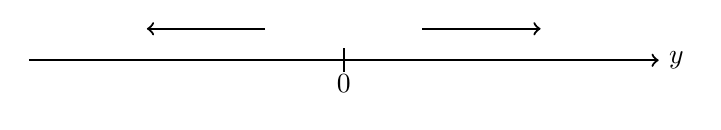
\begin{tikzpicture}

        % 1. Disegna la retta orizzontale orientata (asse principale)
        \draw[->, thick] (-4,0) -- (4,0) node[right] {$y$};

        % 2. Segna lo zero con una piccola tacca verticale
        \draw[thick] (0,-0.15) -- (0,0.15) node[below=0.2cm] {$0$};

        % 3. Freccia a destra che punta verso lo zero (es. limite da destra)
        \draw[->, thick]  (1, 0.4) -- (2.5, 0.4);

        % 4. Freccia a sinistra che punta verso lo zero (es. limite da sinistra)
        \draw[->, thick]  (-1, 0.4)--(-2.5, 0.4);

    \end{tikzpicture}
    \caption{Equilibrio Instabile}
\end{figure}

	Prendiamo ora in considerazione $ \begin{cases}
		\dot Y = -Y\\
		Y(0) = Y_0
	\end{cases}$ che ha soluzione \\
	$Y(t) = y_0e^{-t}$ \\
	\documentclass{article}
\usepackage{tikz}


\begin{figure}[h]
    \centering
    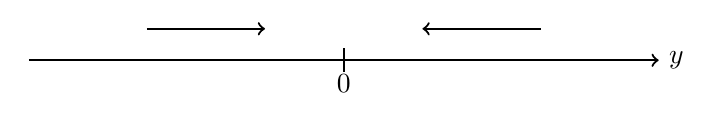
\begin{tikzpicture}

        % 1. Disegna la retta orizzontale orientata (asse principale)
        \draw[->, thick] (-4,0) -- (4,0) node[right] {$y$};

        % 2. Segna lo zero con una piccola tacca verticale
        \draw[thick] (0,-0.15) -- (0,0.15) node[below=0.2cm] {$0$};

        % 3. Freccia a destra che punta verso lo zero (es. limite da destra)
        \draw[->, thick] (2.5, 0.4) -- (1, 0.4);

        % 4. Freccia a sinistra che punta verso lo zero (es. limite da sinistra)
        \draw[->, thick] (-2.5, 0.4) -- (-1, 0.4);

    \end{tikzpicture}
    \caption{Equilibrio Stabile}
\end{figure}
Prendiamo ora in considerazione il sistema della mappa logistica
\[
\begin{cases}
	\dot y = y(1-y) = f(y)\\
	y(0) = 0
\end{cases}
.\] 
Questo ha due punti di equilibrio, $y_0 = 0$ e $y_0 = 1$ tali che $f(y) = 0$\\
Proviamo ora a sviluppare con Taylor attorno ai punti di equilibrio, al primo ordine, avendo così un approssimazione lineare.
\[
	f(y) = y(1-y) = y - y^2 \ \ \substack{\text{vicino a 0}\\\sim} \ \ y
.\] 
Ma questo è un caso che sappiamo trattare\\
    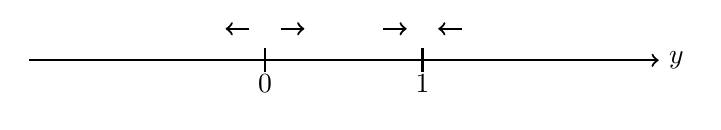
\begin{tikzpicture}

        % 1. Disegna la retta orizzontale orientata (asse principale)
        \draw[->, thick] (-4,0) -- (4,0) node[right] {$y$};

        % 2. Segna lo zero con una piccola tacca verticale
        \draw[thick] (-1,-0.15) -- (-1,0.15) node[below=0.2cm] {$0$};
        \draw[thick] (1,-0.15) -- (1,0.15) node[below=0.2cm] {$1$};

        % 3. Freccia a destra che punta verso lo zero (es. limite da destra)
        \draw[->, thick]  (-0.8, 0.4) -- (-0.5, 0.4);

        % 4. Freccia a sinistra che punta verso lo zero (es. limite da sinistra)
        \draw[->, thick]  (-1.2, 0.4)--(-1.5, 0.4);

        \draw[->, thick]  (0.5, 0.4) -- (0.8, 0.4);

        % 4. Freccia a sinistra che punta verso lo zero (es. limite da sinistra)
        \draw[->, thick]  (1.5, 0.4)--(1.2, 0.4);
    \end{tikzpicture}
    \[
    f(y) \sim f(y_1) + f'(y_1)(y-y_1) + O(|y-y_1|)
    .\] 
    \[
     = 0 + (1 - 2y_1)(y-y_1) + O(|y-y_1|) = -(y-1) = 1-y
    .\] 
    INSERISCI Foto della soluzionea 3 marzo 1:57
    \subsection{Stabilità alla variabile}
    Prendo il solito sistema
    \[
	    \begin{cases}
	    \dot y(t) = f(t,y(t)) \ \ t\in [0,T]\\
	    y(0) = y_0
    \end{cases}
    .\] 
    Chiamo ODE$\delta$ il seguente sistema perturbato
    \[
    \begin{cases}
	    \dot z(t) = f(t,z(t) + \delta(t)) \ \ t\in [0,T]\\
	    z(0) = y_0 + \delta_0
    \end{cases}
    .\] 
    Trovato poiché abbiamo perturbato gli unici due dati del problema, questo può capitare, possiamo vederlo come l'errore causato da uno strumento.\\
    \begin{defi}[Stabilità di Lyapunov]
    ODE è stabile in senso Lyapunov su $(0,T)$ se  $\forall \delta_0$ e $\forall \delta(t)$ tali che  $|\delta_0|< \varepsilon \ \ \ |\delta(t)| < \varepsilon$ per $t\in(0,T)$ con  $\varepsilon > 0$ tale ODE$\delta$ ha  soluzione
    \[
    \exists C > 0 \ \ t.c. |y(t)-z(t)|<C\varepsilon \ \ \forall t\in (0,T)
    .\] 
    \end{defi}
MI RACCOMANDO NON LA SBAGLIARE, ATTENTO AI QUANTIFICATORI \\
Ciò sta a significare che se perturbo poco, le soluzioni sono abbastanza vicine.\\
\begin{defi}
Se $T \rightarrow +\infty$ diciamo che ODE è asintoticamente stabile se:
\begin{enumerate}
	\item è stabile in senso Lyapunov $\forall T> 0$
	\item $|y(t) - z(t)| \xrightarrow{ t \rightarrow +\infty}0$ se $|\delta(t)| \xrightarrow{t \rightarrow+\infty}0$
\end{enumerate}
\end{defi}
\textbf{Esempio:}\\
\[
\begin{cases}
	\dot y = y\\
	y(0) = y_0
\end{cases} \rightarrow \ y(t) = y_0e^t
.\] 
Perturbiamo il sistema nel modo più semplice, perturbiamo il dato iniziale
\[
	\begin{cases}
\dot z = z\\
z(0) = y_0 + \delta_0
	\end{cases}
.\] 
Che ha soluzione $z(t) = (y_0 + \delta_0)e^t$\\
\[
|z(t) - y(t)| = |(y_0 + \delta_0)e^t - y_0e^t| = |\delta_0 e^t| = |\delta_0|e^t\leq |\delta_0|e^T
.\] 
Chiamo $C = e^T$ e ottengo
 \[
|z(t) -y(t)| \leq |\delta_0|C\leq C \varepsilon
.\] 
Ma $e^T$ è enorme, ciò vuol dire che regolare l'errore devo prendere un  $\varepsilon$ minuscolo.\\
La distanza tuttavia non tende a $0$ se $t \rightarrow +\infty$, quindi non abbiamo stabilità asintotica.\\
Quindi questo è stabile in senso di Lyapunov ma non asintoticamente stabile.\\
\textbf{Esempio:}
\[
\begin{cases}
	\dot y = -y\\
	y(t) = y_0
\end{cases} \rightarrow y(t) = y_0e^{-t}
.\] 
\[
\begin{cases}
	\dot z = -z\\
	z(t) = y_0 + \delta_0
\end{cases}
.\]
E otteniamo così
\[
	|z(t) - y(t)| = |\delta_0e^{-t}| = |\delta_0|e^{-t}\leq |\delta_0|= C\varepsilon
.\] 
con $C = 1$
\begin{lemm}[di Gronwall]
	Sia $p$ una funzione integrabile e non negativa su $(0,T)$  e siano  $g, \varphi$ funzioni continue su $[0,T]$ con  $g$ non decrescente.\\
	Se $ \varphi$ soddisfa $ \varphi(t) \leq g(t) + \int_0^Tp(s) \varphi(s)ds \ \ \forall t\in [0,T]$\\
	allora
	\[
		\varphi(t)\leq g(t)e^{\int_0^t \varphi(s) ds} 
	.\] 
\end{lemm}
La dimostrazione è noiosa e la puoi cercare su wikipedia.\\
Considero
\[
\begin{cases}
	\dot y = f(y(t))\\
	y(0) = y_0
\end{cases} \rightarrow y(t) = y_0 + \int_0^tf(y(s))ds
.\] 
Ed è come se avessimo un minore uguale
\[
\begin{cases}
	\dot y \leq f(y(t))\\
	y(0) = y_0
\end{cases} \rightarrow y(t) \leq y_0 + \int_0^tf(y(s))ds
.\] 
La soluzione dell'ODE con la disuguaglianza sta sotto alla soluzione dell'uguaglianza.
\begin{teo}
	Se la dinamica $f$ di ODE è Lipschitziana in $y$ uniformemente in $t$, allora ODE è stabile in senso di Lypaunov.
\end{teo}
\begin{dimo}
	Sia $w(t):= z(t) - y(t)$ con  $z(t)$ soluzione di ODE$\delta$ e $y(t)$ soluzione di ODE.
	\begin{gather*}
	\dot w(t) = \dot z(t) - \dot y(t) = f(t,z(t) + \delta(t)) - f(t,y(t))\\
	 w(0) = z(0) - y(0) = y_0 + \delta_0 - y_0 = \delta_0
	\end{gather*}
	$w$ soddisfa
	\[
		\begin{cases}
	\dot w(t) = f(t,z(t)) - f(t,y(t)) + \delta(t)\\
			w(0) = \delta_0
		\end{cases}
	.\] 
	Sappiamo che $w$ soddisfa
	\[
	|w(t)| = \left|\delta_0 + \int_0^t(f(s,z(s)) - f(s,y(s)) + \delta(s)))ds\right|
	\]
	\[
	\leq |\delta_0| + \left|
\int_0^t(f(s,z(s)) - f(s,y(s)) + \delta(s)))ds\right|
	\] 
	\[
	\leq |\delta_0| + \int_0^t|f(s,z(s))-f(s,y(s))|ds + \int_0^t|\delta(s)|ds
	\] 
	\[
	\leq |\delta_0| + \int_0^tL| z(s)-y(s)|ds + \varepsilon t
	\] 
	\[
	|w(t)|\leq \int_0^tL|w(s)|ds + \varepsilon (t + 1)
	.\] 
	chiamo $\varphi(s) = |w(s)|$ e  $g(t) = \varepsilon(t+1)$, Queste soddisfano le ipotesi del lemma di Gronwall\\
	$ \Rightarrow  $ $|w(t)|\leq \varepsilon(1+t)e^{Lt}\leq \varepsilon (1+T)e^{LT}$ chiamando $C = (1+T)e^{LT}$
\end{dimo}
\textbf{Nota:}\\
Come nel conto di prima questa non garantisce la asintotica stabilità.

\newpage
\part{Metodi Lezione 3}
% --- Content from Lezione_03 ---
	\subsection{Notazioni}
	$y$ è la soluzione esatta di ode 
	\[
	\begin{cases}
		\dot y (t) = f(t,y(t)) \ \ \ t\in (0,T)\\
		$y(0) = y_0$
	\end{cases}
	.\] 
	con $y:(0,T) \rightarrow \R, \ \ f : (0,T)\times \R \rightarrow \R$\\
	La griglia di calcolo su $[0,T]$ con passo uniforme  $h > 0$ è la partizione di ampizza  $h$ del suddetto intervallo\\
	Una volta assegnato $h$ avrò $\lfloor \frac T h \rfloor = : N$ intervalli in  $[0,T]$\\
	Se si assegna  $N$ avrò $\frac T{N-1} = h$\\
	Definiamo poi  $t_n:= n\cdot h$ con  $n = 0,\ldots, N$\\
	Scriviamo infine  $y_n = y(t_n)$ con  $n= 0,\ldots, N-1$ e l'approssimazione numerica di  $y$ sulla griglia come $u_n\approx y_n = y(t_n)$ con  $n = 0,\ldots, N-1$\\
	Chiaramente  $u_n$ è legata ad $h$ e vogliamo che $u_n \xrightarrow {h \rightarrow 0}y_n$\\
	Sappiamo poi che $u_0 \approx y_0$, sarà uguale per i numeri finiti ma per numeri irrazionali sarà solamente simile.\\
	Scriviamo poi $f_n:= f(t_n,u_n)$ (dinamica sulla griglia della soluzione numerica.
	\subsection{Metodi numerici a un passo}
	\begin{defi}
		Un metodo si dice a "un passo" se per calcolare la soluzione al tempo $t_{n+1}$ si usa soltanto la soluzione al tempo $t_n$.\\
		Altrimenti si dice a "più passi" (Multi step)
	\end{defi}
	\begin{defi}
		Un metodo si dice esplicito se il calcolo di $u_{n+1}$ dipende solo da $u_n$ (oppure  $u_{n-1}, u_{n-2},\ldots$) ma non dipende da  $u_{n+1}$, altrimenti si dice implicito
	\end{defi}
	Ad esempio
	\[
		g(x) = 0 \ \ x_{k+1} = x_k - \alpha g(x_k) \ \ se \ \ x_k \xrightarrow{+\infty} x^*
	.\] 
	\[
		x^* = x^* - \alpha g(x^*) \rightarrow g(x^*) = 0
	.\] 
	$g(x_{k+1}) = x_k - \alpha(g_{k+1}) - x_{k+1}$ Metodo implicito.\\
	 \textbf{Esempi}\\
	 $f_n = f(t_n,u_n)$ \\
	 Forward Euler \ \ $u_{n+1} = u_n + hf_n\ \ u_0 = y_0$\\
	 Backward Euelr \ \ $u_{n+1} = u_n + h f_{n+1}$\\
	 Crank-Nicolson \ \  $u_{n+1} = u_n + \frac h 2 (f_n + f_{n+1})$\\
	 Heun \ \  $u_{n+1} = u_n + \frac h 2 (f_n+ f(t_{n+1}, u_n + hf_n))$\\
	 Crank-Nicolson ha calcolo implicito + calcolo esplicito, soluzioni più precise\\


\newpage
\part{Lezione 4 Metodi Numerici}
% --- Content from Lezione_04 ---
	\subsection{Primi schemi}
	usando $f_n = f(t_n,u_n)$\\
	$FE\ \ \ u_{n+1} = u_n + hf_n$\\
	$BE \ \ \ u_{n+1} = u_n + hf_{n+1}$\\
	$CN \ \ \ u_{n+1} = u_n + \frac h 2 (f_n  + f_{n+1})$\\
	$H \ \ \ \ \ u_{n+1} = u_n + \frac h 2 (f_n + f(t_{n+1}, u_n + h f_n))$\\
	Tutti questi metodi hanno una filosofia comune
	\subsection{Filosofia}
	\[
		(ODE) \begin{cases}
		\dot y(t) = f(t,y(t)) \ t\in (0,T)\\
		y(0) = u_0
	\end{cases} \Leftrightarrow (V)\ y(t) = y_0 + \int_0^t f(s,y(s))ds
	.\] 
	Chiaramente a patto di avere una soluzione abbastanza regolare, se la dinamica è continua e anche la mia soluzione lo è, basterebbe.\\
	Chiamiamo la forma dell'ODE forma forte, e la forma di Volterra forma debole.\\

	Nel caso dell'ODE, cosa posso approssimare? Dato che è tutto dato posso solamente approssimare la derivata $\dot y$. (differenze finite)\\

	Nel caso di Volterra, posso approssimare invece l'integrale. (formule di quadratura)\\

	Ricordando che $\dot y = \lim_{\delta \rightarrow 0} \frac{y(t+\delta) - y(t)}{\delta} \\
	\Rightarrow  \phi(\delta) \xrightarrow{\delta \rightarrow 0} 0 \Rightarrow  \dot y(t) = \lim_{\delta \rightarrow 0} \frac{y(t + \phi(\delta)) - y(t) }{\phi(\delta)}$ è una formulazione equivalente\\
	
	Proviamo a fare una scelta particolare $\delta = h$, ovvero il passo di discretizzazione (quanti nodi ci sono)\\
	 \[
		 \dot y(t) = \lim_{h \rightarrow 0}\frac{y(t+h)-y(t)} h\approx \frac{y(t+h) - y(t)}h
	.\] 
	\textbf{Esempio}\\
	$\lim_{x \rightarrow 0}\frac{\sin x}x$ in matlab se sostituissi la $x$, verrebbe Nan, per ovviare a questo problema possiamo fare lo sviluppo di Taylor
	\[
		\Rightarrow  f(x) \sim f(x_0) + f'(x_0)(x-x_0) + \frac{f''(x_0)} 2 (x-x_0)^2 + \ldots
	.\] 
	$ \Rightarrow  \sin x \sim 0 + x - \frac{x^3}6 + \ldots$ \\
	\[
		\frac{\sin x}x \sim \frac{x - \frac {x^3}6 + O(x^3)}x = 1 - \frac{x^2}6 + o(x^2) \xrightarrow{x \rightarrow 0} 1
	.\] 
	Quindi tornando al nostro rapporto incrementale con $h$ (necessariamente) fissato\\
	\[
		\frac{ y(t+h) - y(t)}h =\frac{ \cancel{y(t)} + y'(t) + \frac 12 h^2y''(\xi) - \cancel{y(t)}}{h}
	.\] 
	con $t < \xi < t+ h$\\
	\[\frac{y(t+h) - y(t)}h = y'(t) + \frac 12 h y''(\xi)\]
	Quindi se approssimo ho un errore proporzionale a $h$
	\[
		err = \left|\frac{y(t+h)-y(t)}h - y'(t) \right| = \frac 12h|y''(\xi)|\leq \frac{M h}2
	.\] 
	con $M = \max_{0 < \xi < h}|y''(\xi)|$ \\
	Se voglio che $\frac{Mh}2 < tol$  dovrò avere  $h < \frac {2 tol} M$\\
	Tornando alla nostra ODE
	\[
	\begin{cases}
		\dot y(t) = f(t,y(t))\\
		y(0) = y_0
	\end{cases} \rightarrow \frac{y(t+h) + y(t)}h = f(t,y(t))
	.\] 
	Leggiamo questa espressione con $t = t_n\ \ n = 0,\ldots, N$
	 \[
		 \frac{y(t_n + h) - y(t_n)}h = f(t_n,y(t_n))
	.\] 
	ovvero $y(t_{n+1}) = y(t_n) + hf(t_n,y(t_n))$, il metodo di Eulero in avanti\\

	Posso ora provare ad approssimare la derivata prima in un altro modo.
	 \[
		 \dot y(t) = \lim_{ h \rightarrow 0}\frac{ y(t) - y(t-h)}h
	.\] 
	\[
		\dot y(t) = f(t,y(t)) \rightarrow \frac{y(t) - y(t-h)}h = f(t,y(t))
	.\] 
	$y(t) = y(t-h) + h f(t,y(t))$\\
	Leggo in $t = t_{n+1} \Rightarrow  y(t_{n+1} = y(t) + hf(t_{n+1},y(t_{n+1}))$ ovvero Eulero all'indietro.\\
	Cambiamo punto di vista:\\
	$y(t) = y_0 + \int_0^tf(s,y(s))ds$\\
	Posso approssimare con dei quadrati $\int_0^t f(s,y(s))ds\sim tf(0,y(0))$\\
	Scriviamo ora la forma di volterra in $t+h$
	 \[
		 y(t+h) =y_0 + \int_0^{t+h}f(s,y(s))ds = y_0 + \int_0^tf(s,y(s))ds + \int_{t}^{t+h}f(s,y(s))ds
	.\] 
	se $y = t_n$
	 \[
		 y(t_n + h) = y(t_{n+1}) = y_0 + \int_0^{t_n}f(s,y(s))ds + \int_{t_n}^{t_{n+1}}f(s,y(s))ds
	\] 
	\[
	 = y(t_n) + \int_{t_n}^{t_{n+1}}f(s,y(s))ds
	.\] 
	\[
		y(t_{n+1}) = y(t_n) + \int_{t_n}^{t_{n+1}}f(s,y(s))ds
	.\] 
	Approssimazione con il metodo dei rettangoli (a sinistra)
	\[
		\int_{t_n}^{t_{n+1}} f(s,y(s))ds\sim h f(t_n,y(t_n))
	.\] 
	Ovvero Eulero in avanti\\
	Approssimazione con il metodo dei rettangoli (a destra)
	\[
		\int_{t_n}^{t_{n+1}}f(s,y(s))ds \sim hf(t_{n+1},y(t_{n+1}))
	.\] 
	Ovvero Eulero all'indietro\\
	Approssimazione con il metodo dei trapezi
	\[
		\int_{t_n}^{t_{n+1}}f(s,y(s))ds\sim \frac h 2 (f(t_n,y(t_n)) + f(t_{n+1},y(t_{n+1})))
	.\] 
	Ovvero Crank Nicholson\\
	Heun la vediamo dopo, non utilizza valori della griglia.\\
	Introduciamo il $\theta$-Metodo,\\
	Scelgo $\theta\in [0,1]$
	 \[
		 \int_{t_n}^{t_{n+1}}f(s,y(s))ds \sim h \left((1-\theta)f(t_n,y(t_n)) + \theta f(t_{n+1},y(t_{n+1})) \right)
	.\] 
	Per $\theta = \frac 12 $ ottengo Crank Nicholson.\\
	Cosa succede se
	 \[
	 	 \frac{y(t+h) - y(t-h)}{2h} = \frac{y(t + h) - y(t) + y(t) - y(t+h)}{2h} 
	\] 
	\[
		= \frac 12 \left(\frac{y(t+h)-y(t)}h \right) + \frac 12  \left( \frac{y(t) - y(t-h)}h \right) \xrightarrow{h \rightarrow 0} \frac 12\dot y(t) + \frac 12 \dot y(t) = \dot y(t)
	.\]
	Questo metodo ci permette di semplificare i termini di ordine superiore nello sviluppo di Taylor.\\
	Faccio lo sviluppo di Taylor di $y(t+h)$ in  $t$ \\
	\[
	y(t+h) = y(t) + \dot y(t)h + \frac 12 \ddot y(t)h^2 + \frac 16 \dddot y(\xi)h^3\ \ t < \xi < t + h
	.\] 
	\[
	y(t-h) = y(t) - \dot y(t)h + \frac 12 \ddot y(t)h^2  - \frac 16\dddot y(\eta)h^3\ \ \ t-h < \eta < t 
	.\] 
	Facendo la differenza rimuovo i termini pari
	\[
	y(t+h) - y(t-h) = \dot y(t)2h + \frac 16 h^3(\dddot y(\xi) + \dddot y(\eta))
	.\] 
	Dividendo entrambe le parti per $2h$
	 \[
		 \frac{y(t+h)-y(t-h)}{2h} = \dot y(t) + \frac{h^2}{12}(\dddot y(\xi) + \dddot y(\eta))
	.\] 
	Possiamo quindi essere più precisi, ma al costo di utilizzare dei nodi diversi, utilizza non solo $t_{n}$ ma anche  $t_{n-1}$, ovvero è uno schema a 2 passi.\\
	$\dot y(t) = f(t,y(t)) \Rightarrow  \frac{y(t+h) - y(t-h)}{2h} = f(t,y(t))$ \\
	$t=t_n$
	 \[
		 \frac{y(t_{n+1}) - y(t_{n-1})}{2h} = f(t_{n},y(t_{n})) \Rightarrow  y(t_{n+1}) = y(t_{n-1}) + 2h f(t_n,y(t_n))
	.\] 
	Questo è un metodo esplicito a 2 passi, viene chiamato il mid-point, poichè dal punto di vista integrale è come se approssimassimo gli integrali con li quadrato di base il punto medio\\
	\[
		y(t+h) = y(t) + \int_{t_n}^{t_{n+1}}f(s,y(s))ds = y(t-h) + \int_{t-h}^tf(s,y(s))ds + \int_t^{t+h}f(s,y(s))ds
	\] \[
	= y(t-h) + \int_{t-h}^{t+h}f(s,y(s))ds
	.\] 
	\subsection{Analisi dei metodi ad un passo (espliciti)}
\[
	u_{n+1} = u_n + h\Phi(t_n,u_n; h, f)
.\] 
il punto e virgola è per dire che in generale deve dipendere da $h$ e dalla dinamica del problema.\\
$\Phi$ è la funzione incremento.\\
 \textbf{Esempi}\\
 $\Phi(t_n,u_n) = f(t_n,u_n)$ \hfill  (FE)\\
 $\Phi(t_n,u_n) = \frac 12 (f(t_n,u_n) + f(t_{n+1},u_n + hf(t_n,u_n)))$ \hfill (H)
 \subsubsection{Consistenza}
Se sostituisco la soluzione esatta di ODE nello schema commetto un errore
\[
	y(t_{n+1}) = y(t_n) + h\Phi(t_n,y(t_n))+ \varepsilon_{n+1}
.\] 
o come formulazione alternativa
\[
	\varepsilon_{n+1}:= y(t_{n+1})-y(t_n) -h \Phi(t_n,y(t_n))
.\] 
Chiamo $\varepsilon_{n+1}$ residuo al tempo  $t_{n+1}$\\
Riscrivo $\varepsilon_{n+1} = hz_{n+1}(h)$ LTE (Local Truncation Error)


\newpage
\part{Lezione 05 Metodi}
% --- Content from Lezione_05 ---
	\subsection{Consistenza di un metodo a un passo per ODE}
	\[
	\begin{cases}
		\dot y(t) = f(t,y(t))\\
		y(0) = y_0
	\end{cases}
	.\] 
	Per approssimare la soluzione esatta $y(t)$ utilizziamo il seguente schema
	\[
	\begin{cases}
		u_{n+1} = u_n +h \Phi(t_n, u_n; h,f)\\
		u_0 \approx y_0
	\end{cases}
	.\] 
	Possiamo immaginare quindi $\Phi$ come una scatola nera che ci restituisce il nodo successivo della nostra approssimazione.\\
	Definiamo ora la consistenza:\\
	Uno schema numerico si dice consistente se approssiam l'equazione differenziale.\\
	\textbf{Osservazione}\\
	$y_n + h\Phi(t_n,y_n)\substack{?\\=}y_{n+1}$?\\
	non necessariamente, poiché  $y_{n+1} = y(t_{n+1})$ e potrebbe non avere relazioni con l'approssimazione dello schema.\\
	\begin{defi}[Residuo]
	\[\varepsilon_{n+1} := y_{n+1} - (y_n + h\Phi(t_n,y_n).\]
	\end{defi}
	voglio quindi che $\varepsilon_{n+1} \xrightarrow{h \rightarrow 0}0$ \ \ $\forall n$\\
	Scriviamo quindi
	 \[
		 \frac{y_{n+1}-(y_n + h \Phi(t_n,y_n))}h= \frac{\varepsilon_{n+1}}{h} \Rightarrow \frac{y_{n+1}-y_n}{h} - \Phi(t_n,y_n) = \frac{\varepsilon_{n+1}}h = \tau_{n+1}
	.\] 
Da cui deduciamo che se il metodo è consistente allora.
\[
	\lim_{h \rightarrow 0 }\Phi(t_n,y_n) = f(t_n,y_n)
.\] 
$t_{n+1}(h) = \frac{\varepsion_{n+1}}h$ è l'errore locale di troncamento.\\
Una definizione equivalente è
 \begin{defi}
	Il metodo si dice consistente se 
	\[
		\tau_{n+1}(h) \xrightarrow{h \rightarrow 0} 0 \ \ \forall n = 0,\ldots, N-1
	.\]  
	Se $\tau_{n+1} = O(h^q)$ con  $q\geq 1$, il metodo si dice consistente di ordine  $q$.
\end{defi}
\textbf{Esempio}\\
Eulero in avanti:\\
$u_{n+1} = u_n + hf(t_n,u_n)$ con  $\Phi(t_n,u_n):= f(t_n,u_n)$\\
$\varepsilon_{n+1}= h\tau_{n+1}(h) = y_{n+1}-y_n-hf(t_n,y_n) = y(t_n + h) - y(t_n) - hf(t_n,y(t_n))$\\
Usando lo sviluppo di Taylor di  $y(t_n + h)$ in  $t_n$ otteniamo
 \[
	 h\tau_{n+1}(h) = \cancel{y(t_n)} + \cancel{\dot y(t_n)h} + \frac 12 \ddot y(\xi)h^2 - \cancel{y(t_n)} - \cancel{hf(t_n,y(t_n))}; \text{ con } \xi\in(t_n, t_n + h)
.\] 
Quindi 
\[
	h\tau_{n+1}(h) = \frac 12 \ddot y(\xi)h^2 \Rightarrow  \tau_{n+1}(h) = \frac 12\ddot y(\xi)h
.\]  
$ \Rightarrow  |\tau_{n+1}(h)|\leq \frac 12 Mh;$ dove $M = \max_{t\in[0,T]}|\ddot y(t)|$ \  $\forall n$\\
\begin{defi}[GTE (Global Truncation Erorr)]
	\[
		\tau(h) = \sup_{n}|\tau_{n+1}(h)|
	.\] 
\end{defi}
\textbf{Crank-Nicolson}
\[
	u_{n+1} = u_n + \frac h 2(f(t_n,u_n) + f(t_{n+1}, u_{n+1}))\\
.\] 
$h\tau_{n+1}(h) = y_{n+1} - y_n - \frac h 2 (f(t_n,y_n) + f(t_n,y_{n+1}))$\\
Uso lo sviluppo di Taylor\\
$y_{n+1} = y(t_n + h) = y(t_n) + \dot y(t_n) h + \frac 12 \ddot y(t_n)h^2 + \frac 16 \dddot y (\xi) h^3$, \ \ $\xi \in (t_n,t_{n+1})$\\
 \textbf{Nota}\\
 $f(t_n + h, y(t_n + h):= g(h)$ dato che  $t_n$ è fisso a me interessa lo sviluppo per $h \rightarrow 0$\\
 \[
 g(h) = g(0) + g'(0) h + O(h^2)
 .\] 
 con $g(0) = f(t_n,y_n)$ \\
\[
	g'(h) = \drac{\partial f}{\partial t}(t_n+h,y(t_n+h)) + \frac{\partial f}{\partial y} (t_n+h,y(t_n+h))\dot y(t_n+h)
\] 
\[
	\Rightarrow g'(0) = \frac{\partial f}{\partial t}(t_n,y(t_n)) + \frac {\partial f}{\partial y}(t_n,y(t_n))\dot y(t_n)
.\] 
Possiamo quidni scrivere
\[
	f(t_n+h,y(t_n+h)) = f(t_n,y(t_n)) + (\frac{\partial f}{\partial t}(t_n,y(t_n)) + \frac{\partial f}{\partial t} (t_n,y(t_n))f(t_n,y(t_n))h + O(h^2)
.\] 
Quindi:\\
\[
	\begin{split}
		h\tau_{n+1}(h) & = y_{n+1}-y_n-\frac h 2(f(t_n,y_n) + g(t_{n+1}y_{n+1}))\\
			       & =y_n + \dot y_n + h\ddot y_n h^2 + O(h^3) - y_n - \frac h 2 f_n - \frac h 2 \left[ f_n + \left(\frac{\partial fn}{\partial t} + \frac {\partial f_n}{\partial y}f_n \right)h + O(h^2)\right]
	\end{split}
.\] 
\[
	\Rightarrow  h\tau_{n+1}(h) = \frac 12 \left(\frac{\parital f_n}{\partial t} + \frac{\partial f_n}{\partial y} f_n \right) h^2+ O(h^3) - \frac {h^2}2 \left(\frac {\partial f_n}{\partial t} + \frac{\partial f_n}{\partial y}f_n \right)h^2 + O(h^3)
.\] 
\[
	\Rightarrow  h\tau_{n+1}(h) = O(h^3) \Rightarrow  \tau_{n+1}(h) = O(h^2)
.\] 
Quindi facendo
\[
\tau(h) = \sup_n|\tau_{n+1}(h)| =  O(h^2)
.\] 
\textbf{Esercizio}\\
Calcolare la consistenza del metodo di Heun
\[
	u_{n+1} = u_n + \frac {h} 2 [f(t_n,u_n) + (u_n + h(f(t_n,u_N))]
.\] 

\newpage
\part{Lezione 6 Metodi numerici}
% --- Content from Lezione_06 ---
	\section{Zero Stabilità }
	(Parallelo alla stabilità di Lyapinov)\\
	La stabilità di Lyapinov riguarda gli ODE, la \textbf{zero-stabilità} è una proprietà dello schema, non dell'ODE che sto approssimando.\\

	Sia $\{u_n\}$ la soluzione numerica di  $ \begin{cases}
		u_{n+1} = u_n + h\Phi(t_n,u_n; h, f)\\
		 u_0 = y_0
	\end{cases}$\\
	
	Sia $\{z_n\}$ la soluzione (numerica) di  $ \begin{cases}
		z_{n+1} = z_n + h[ \Phi(t_n,z_n;h,f) + \delta_{n+1}]\\
		z_0 = y_0 + \delta_0

	\end{cases}$
	$0\leq n\leq N-1 \ \ N = N(h) = [\frac T H]$\\
	Il professore dice che sti quantificatori li sbagliano tutti, stai attento
	 \begin{defi}
		Diciamo che il metodo è zero-stabile se\\
		$\exists h_0 > 0, \exists C>0$ tale che $\forall h \in (0,h_0]$ e $\forall \varepsilon > 0 $ sufficientemente piccolo se  $|\delta_{n+1}| < \varepsilon$  per  $0\leq n \leq N-1$ e  $|\delta_0| < \varepsilon$, allora
		\[
			|z_n^{(h)}-u_n^{(h)}|\leq C\cdot \varepsilon \ \ \ 0\leq n\leq N
		.\] 
	\end{defi}
	l'h come apice sta a significare che $z_n$ e $u_n$ dipendono da $h$, nonostante ciò sono tutte controllate dalla stessa costante.

	\begin{lemm}[di Gronwall discreto]
		Sia $p_n$ una successione non negativa e siano $g_n, \varphi_n$ successioni con $g_n$ non decrescente\\
		Se  $ \varphi_n$ soddisfa $ \varphi_n\leq g_n + \sum^{k=0}_{n-1}p_k \varphi_k\ \ \forall n\geq 0$, allora $ \varphi_n \leq g_n exp( \sum^{k=0}_{n-1}p_k )$
	\end{lemm}
	La dimostrazione è noiosa.\\
	\begin{teo}
		Se la funzione incremento $ \Phi$ è Lipschitziana nella variabile $u_n$ uniformemente in  $t_n$ con costante di Lipschitiz  $\Lambda$ (indipendente dai nodi  $t_n$ e da $h$) allora il metodo  $u_{n+1} = u_n + h\Phi(t_n,u_n)$ è zero-stabile
	\end{teo}
	\textbf{Reminder}\\
	funzione Lipschitizna nelal variabile $u_n$ uniformemente in $t_n$
	\[
		\exists h_0 > 0, \exists \Lambda > 0, \ t.c. \ \forall h\in (0,h_0]
	.\] 
	 \[
	|\Phi(t_n,u_n) - \Phi(t_n,z_n)| \leq \Lambda |u_n - z_n|
	.\] 
	\textbf{Osservazione:}\\
	Cado del metodo di Heun
	\[
		u_{n+1} = u_n + h/2(f(t_n,u_n) + f(t_{n+1},u_n + hf(t_n,u_n)))
	\] 
	\[
		\Rightarrow  \Phi(t_n,u_n) = \frac 12 f(t_n,u_n) + \frac 12 f(t_{n+1},u_n + h f(t_n,u_n))
	.\] 
	Proviamo a trovare $\Lambda$.\\
	Valutiamo
	 \[
	 | \Phi(t_n,u_n)- \Phi(t_n,z_n)| = \]\[=\left|\frac 12 f(t_n,u_n) + \frac 12 (t_{n+1},u_n + h f ( t_n,u_n)) - \frac 12 (t_n,z_n) - \frac 12 f(t_{n+1},z_n + h f(t_n,z_n))\right|
	.\] 
	Con la disugualgianza triangolare
	\[
		\leq \frac 12 \left| f(t_n,u_n)-f(t_n,z_n)\right| + \frac 12 \left| f(t_{n+1},u_n+ hf(t_n,u_n)) - f(t_{n+1},z_n+hf(t_n,z_n))\right|
	\] 
	e tramite la Lipschitzianità
	\[
	\leq \frac 12 L|u_n-z_n| + \frac 12 L |u_n + hf(t_n,u_n)-z_n-hf(t_n,z_n)|
	.\] 
	\[
	\leq \frac 12 L|u_n-z_n| + \frac 12 L(|u_n-z_n| + h |f(t_n,u_n) - f(t_n,z_n)|)
	\] 
	\[
	\leq \frac 12 L|u_n-z_n| + \frac 12 L|u_n-z_n| + \frac 12 LhL|u_n-z_n|
	\] 
	\[
	\Rightarrow  |\Phi(t_n,u_n)-\Phi(t_n,z_n)|\leq (L + \frac 12 L^2h)|u_n-z_n| = L(1+\frac 12 Lh)|u_n-z_n|
	\] 
	Ponendo $h_0 = 1$
	\[
	\leq L(1 + \frac 12 L h_0)|u_n-z_n|
	.\] 
	Posso quindi chiamare $\Lambda = L(1 + \frac 12 Lh_0)$
	\begin{dimo}
	Definiamo $w_k = z_k - u_k $ e otteniamo i corrispondneti schemi\\
	$u_{k+1} = u_k + h\Phi(t_k,u_k)\ \ u_0 = y_0$\\
	$z_{k=1} = z_k + h[\Phi(t_k,z_k) + \delta_{k+1}]\ \ \ z_0 = y_0 + \delta_0$\\
	Sottraiamo membro a membro
	\[
		z_{k+1} - u_{k+1} = z_k - u_k + h\delta_{k+1} + h( \Phi(t_n,z_n)-\Phi(t_k,u_k))\ \ z_0 - u_0 = y_0 + \delta_0- y_0 = \delta_0
	.\] 
	Ovvero
	\[
		w_{k+1} = w_k + h(\Phi(t_k,z_k) - \Phi(t_k,u_k)) + h\delta_{k+1}
	.\] 
	Ora se $\Phi$ fosse lineare avremmo $\Phi(t_k,z_k-u_k) = \Phi(t_k,w_k)$ avremmo quindi avuto lo schema per $w_k$, tuttavia non possiamo, dobbiamo quindi fare delle stime
	Scelgo $n$ e sommo su $ k$ da $0$ a $n-1$
	 \[
		 \sum^{n-1}_{k=0}w_{k+1} = \sum^{n-1}_{k=0}w_k + h \sum^{n-1}_{k=0}(\Phi(t_k,z_k) - \Phi(t_k,u_k)) + h \sum^{n-1}_{k=0}\delta_{k+1}
	.\] 
	Riscrivo come
	\[
		\cancel{\sum^{n-1}_{k=1}w_k} +w_n = w_0 + \cancel{\sum^{n-1}_{k=1}w_k} + h\cdots
	\] 
	\begin{aligned}
		$|w_n| &= \left|w_0 + h \sum^{n-1}_{k=0}(\Phi(t_n,z_n) - \Phi(t_k,u_k)) + h \sum^{n-1}_{k=0}\delta_{k+1}\right|$\\
		$ &\leq |w_0| + h \left| \sum^{n-1}_{k=0}(\Phi(t_k,z_k)-\Phi(t_k,u_k))\right| + h \sum^{n-1}_{k=0}|\delta_{k+1}|$\\
		$ &\leq |w_0| + h  \sum^{n-1}_{k=0}\left|(\Phi(t_k,z_k)-\Phi(t_k,u_k)\right|) + h \sum^{n-1}_{k=0}|\delta_{k+1}|$\\
		$ &\leq |w_0| + h  \sum^{n-1}_{k=0}\left|(\Phi(t_k,z_k)-\Phi(t_k,u_k)\right|) + h \sum^{n-1}_{k=0}|\delta_{k+1}|$\\
	\end{aligned}
	otteniamo quindi
	\[
		|w_n|\leq |w_0|  + h \sum^{n-1}_{k=0}\Lambda|z_k-u_k| + h \sum^{n-1}_{k=0}|\delta_{k+1}|
	.\] 
	$p_n := h\Lambda$, \ \ $g_n = \begin{cases}
		|w_0| \ \ \text{se } n= 0\\
		|w_0| + h \sum^{n-1}_{k=0}|\delta_{k+1}| \ \text{ se } n\geq 1
	\end{cases}$
	$ \varphi_n = |w_n|, \\
	\varphi_n\leq g_n + \sum^{n+1}_{k=0}p_n \varphi_n$ $ \Rightarrow  \varphi_n\leq g_nexp \left( \sum^{n-1}_{k=0}p_k \right)$\\
	ovvero 
	\[
		|w_n|\leq \left( |w_0| + h \sum^{n-1}_{k=0}|\delta_{k+1}| \right)exp \left( \sum^{n-1}_{k=0}h\Lambda \right)
	.\] 
	per ipotesi
	\[
		|\delta_k| < \varepsilon\ \ \text{ per ogni } k
	.\] 
	e quindi
	\[
	\leq \left(\varepsilon +h \sum^{n-1}_{k=0} \varepsilon \right) exp \left( nh\Lambda \right)\leq  \left(\varepsilon +h n\varepsilon \right) exp(nh\Lambda)
	.\] 
	Segue quindi 
	\[
		|w_n|\leq \varepsilon(1 + hn)exp(nh\Lambda)
	.\] 
	\[
	|w_n| \leq \varepsilon (1 + t_n)e^{t_n\Lambda}
	.\] 
	ma sappiamo che $t_n\leq T$ per ogni $n$, guardando ora i singoli pezzi\\
	$e^{t_n\Lambda}\leq e^{T\Lambda}$ l'esponenziale è crescnete\\
	$1 + t_n\leq 1 + T$ 
	\[
		|z_n-u_n|=|w_n| \leq \varepsilon (1+T)e^{T\Lambda} = C\varepsilon
	.\] 
	\end{dimo}
	Notiamo che la costante $C$ è la stessa del continuo, dipende solamente dal sistema.\\
	Questo risultato è fondamentale per l'analisi numerica, $z_n$ è il perturbato del problema, quello che effettivamente posso scrivere al computer.\\
Se questa proprietà non ci fosse non potrei implementare nulla, il mio $z_n$ potrebbe non rimanere vicino a $u_n$.\\
È come se ci fossero 3 livelli, il primo della relatà, dove  $\pi$ non esiste, il seocondo dell'analisi numerica, dove posso fare stime su uno schema risolutivo, e il terzo dove vive la vera soluzione del problema differenziale.\\

Sostanzialmente la consistenza mi dice che lo schema che considero approssima l'ODE.\\

La zero-stabilità mi dice che lo schema accumula errore in modo controllato.\\

Mi manca l'ultimo step delal convergenza, $u_n \xrightarrow{h \rightarrow 0} y_n?$


\newpage
\part{Lezione 7 Metodi}
% --- Content from Lezione_07 ---
	\section{Convergenza}
	\subsection{Riassuntino}
	\textbf{Consistenza:} Lo schema approssima l'ODE? Se $Z(h) \rightarrow 0$ (l'errore tende a 0)\\
	o alternativamente $\Phi(t_n,u_n) \xrightarrow{h \rightarrow 0}f(t_n,u_n)$.\\
	Si sostituisce la soluzione esatta $y$ di ODE nello schema e usando sviluppi di Taylor (assumendo che la soluzione sia sufficientemente regolare)\\
	si mostra che  $\tau(h) \rightarrow 0$\\
	Se $y$ è sufficientemente regolare $\tau(h) = O(h^q)$ ($q$ è ordine di consistenza)\\[10px]
	\textbf{Zero-stabilità:} Lo schema è poco sensibile alle perturbazioni.\\
$|u_n-z_n|\leq C|u_0-z_0| = C\varepsilon$   (differenza  tra soluzione perturbata e soluzione non perturbata, controllata dalla differenza iniziale)\\
quindi se $C\varepsilon < tol \Rightarrow  \varepsilon < \frac{tol}C$ \\
Se $C$ diventa molto grande sono costretto ad un  $\varepsilon$ molto piccolo.\\
Se $\Phi$ è Lipschitziana con costante $\Lambda \Rightarrow $ lo schema (il metodo) è zero-stabile.\\
\subsection{Convergenza}\\
$u_n \xrightarrow{ h \rightarrow 0 } y_n$
\begin{defi}[Convergenza]
	Uno schema si dice convergente se $\exists C = C(h)$ tale che 
	\[
		|u_n - y_n|\leq C(h) \ \ \text{ e } \ \ C(h) \xrightarrow{h \rightarrow 0} 0\ \ \ \ 0\leq n\leq N
	.\] 
Se $y$ è sufficientemente regolare  e $C(h) = O(h^r)$ allora il metodo si dice convergente con ordine $r$. Chiameremo $r$ ordine di convergenza.
\end{defi}
\begin{teo}[di equivalenza di Lax-Richtmyer (Dahlquist)]
	Se lo schema numerico è consistente e $|y_0-u_0| \xrightarrow{h \rightarrow 0} 0$ allora è convergente.\\
	Se inoltre $|y_0 - u_0| = O(h^s)$ e lo schema ha ordine di consistenza $O(h^q)$ allora è convergente con ordine  $O(h^{\min\{s,q\}})$
\end{teo}
\textbf{Nota:}\\
$u_0 $ non è $y_0$, per esempio $\pi$ possiamo prendere solo $n$ cifre dopo la virgola, non il valore esatto. La differenza può tendere a $0$ se magari ho una procedura che approssima $\pi$.
 \begin{dimo}
	 Pensiamo $\{y_n\}$ come perturbazione di $\{u_n\}$ 
	 \[
		 u_{n+1} = u_n + h\Phi(t_n,u_n)
	 .\] 
	 \[
		 y_{n+1} = y_n + h\Phi(t_n,y_n) + h \tau_{n+1}(h)
	 .\] 
	 dove $\tay_{n+1}(h)$ è l'errore locale di troncamento.\\
	 Se chiamiamo\ \ $h[\Phi + \delta_{n+1}]$\\
	 $\delta_0 = y_0 - u_0$\\
	 $\delta_{n+1} = \tau_{n+1}(h)$ \\
	 Ripercorrendo la dimostrazione che utilizza il lemma di Gronwall discreto per la zero-stabilità, segue immediatamente
	 \[
		 |y_n - u_n| \leq (|y_0 - u_0| + nh\tau(h))e^{nh\Lambda} \ \ \ nh = t_n \leq T \ \ 0\leq n \leq N
	 .\] 
	 dove $\displaystyle\tau(h) = \sup_{n}|\tau_n(h)|$ \\
	 $ \Rightarrow  |y_n - u_n|\leq (|y_0 - u_0| + T\tau (h))e^{T\Lambda}  = \varepsilon C$ \\
	 dove $\varepsilon = |y_0-u_0 | + T\tau(h)$ e $C = e^{T\Lambda}$ e abbiamo $|y_0-u_0|$ che è l'errore sui dati, $T\tau(h)$ è la consistenza e $e^{T\Lambda}$ è la zero-stabilità\\
	 Usando infine le ipotesi\\
	 se  $| y_0 - u_0| \xrightarrow{h \rightarrow 0} 0$ e $\tau(h) \xrightarrow{ h \rightarrow 0} 0$  allora $|y_n-u_n| \xrightarrow{h \rightarrow 0} 0$ $0 \leq n\leq N$\\
	 Se inoltre $|y_0 - u_0| = O(h^s)$ e $\tau(h) = O(h^q)$ allora l'ordine di convergenza è $O(h^{\min\{q,s\}})$ (Si capisce facilemnte dalla disequaizone sopra, la somma si "mangia" l'ordine maggiore)
\end{dimo}
\textbf{Nota:}\\
Da notare come la richiesta sulla soluzione è solamente la sua esistenza.\\
Consistenza + Zero-Stabilità $ \Rightarrow $ Convergenza\\
\textbf{Analisi esplicita per il metodo di Eulero in avanti}\\
Inizialmente assumiamo $u_0 = y_0$\\
\[
	u_{n+1} = u_n + hf(t_n,u_n)
.\] 
La soluzione esatta risolve $y'(t_n) = f(t_n,y(t_n))$ scriviamo in modo più compatto  $y'_n = f(t_n,y_n)$\\
e  soddisfa
\[
	y_{n+1} = y_n  + hf(t_n,y_n) + h\tau_{n+1}(h)
.\] 
dato che c'è l'errore di troncamento\\
Definiamo 
\[
	u_{n+1}^* = y_n + hf(t_n,y_n) = y_n + h y'(t_n)
.\] 
TODO AGGIUNGI FOTO 20 marzo 11:33\\
L'errore 
 \[
	 e_{n+1} := y_{n+1} - u_{n+1} = (y_{n+1}-u_{n+1}^*) + (u_{n+1}^*- u_{n+1})
\] \[
= h\tau_{n+1}(h) + \alpha
.\] 
dove $\alpha$ è l'accumulazione degli errori precedenti.
\[
	u_{n+1}^*-u_{n+1}= y_n-u_n + h(f(t_n,y_n) - f(t_n,u_n)) = e_n + h(f(t_n,y_n) - f(t_n,u_n))
.\] 
\[
	\Rightarrow  e_{n+1} = h\tau_{n+1}(h) + e_n + h(f(t_n,y_n) - f(t_n,u_n))
.\] 
\[
	|e_{n+1}|\leq h | \tau_{n+1}(h)| + |e_n| + hL |y_n - u_n|\ \ \substack{\leq\\ \sup_n|\tau_{n+1}} \ \ h|\tau(h) | + (1 + hL)|e_n|
.\] 
$e_0 = y_0 - u_0= 0$\\
$|e_1|\leq h|\tau(h)|$, $|e_2|\leq h|\tau(h)| + (1 + hL)|e_1|\leq h|\tau(h) + (1+hL)h|\tau(h)| = h|\tau(h)|(1 + (1 + hL))$\\
$|e_n|\leq h|\tau(h)|[1 + (1 + hL) + (1 + hL)^2 + \ldots + (1 + hL)^{n-1}]$ 
 $\displaystyle = h |\tau(h)|\sum^{n-1}_{k=0}(1+hL)^k$\\
 $ \displaystyle = h|\tau(h)|\frac{1 - (1 + hL)^n}{1 - (1+hL)}= h|\tau(h)|\frac{1 - (1 + hL)^n}{-hL} =h|\tau(h)| \frac{(1 - hL)^n - 1}{hL}$\\
 e utilizzando la stima  $h\leq \frac Tn $\\
 $\displaystyle \leq \frac{(1 + \frac T n L )^n-1}{hL} \leq \frac{e^{LT}-1}{hL}$\\
 \[|e_n|\leq \cancel{h}|\tau(h)|\frac{e^{Lt}-1}{\cancel{h}L}.\]

 $h\tau_{n+1} = y_{n+1} - y_n - hf(t_n,y_n)$\\
 $h\tay_{n+1} = y_n + h y_n' + \frac {h^2}2 y''(\xi_n)- y_n-h f(t_n,y_n) = \frac {h^2}2 y''(\xi_n) \ \ t_n\leq\xi_n\leq t_{n+1}$\\
 $\tau_{n+1} = \frac h 2 y''(\xi_n)$\\
 $\displaystyle|\tau_{n+1}|\leq \frac h 2 \sup_{t}|y''(t)| = h \frac M 2$ \\
 con $M = \sup_t|y''(t)|$\\
 In conclusione
  \[
	  |e_n|\leq h\frac M 2 \frac{e^{LT} - 1}L = h C
 .\] 
 con $C = \frac M 2 \frac{e^{LT} - 1}L$ \\
 Quindi Eulero fa schifo perché è di ordine 1 ma $C$ può essere molto grande.\\
 Vedremo il caso in cui i dati non son esatti.



\newpage
\part{Lezione 8 Metodi Numerici}
% --- Content from Lezione_08 ---
	Prendiamo in considerazione
	\[
	\begin{cases}
		\dot y(t) = f(t,y(t)) \ \ \ t\in (0,T)\\
		y(0) = y_0
	\end{cases} \Rightarrow  y_{n+1} = y_n + h\Phi(t_n,y_n) + h\tau_{n+1}(h)
	.\] 
	\[
		\begin{cases}
			\bar u_{n+1} = \bar u_n + h \Phi(t_n,U\bar u_n) + \xi_{n+1} = \bar u_n + h[\Phi(t_n,\bar u_n) + \frac {\xi_{n+1}} {h} ]\\
		\bar u_0 = y_0 + \xi_0
		\end{cases}
	.\] 
	dove $\xi_{n+1}$ sono gli errori dovuti all'aritmetica finita.
	Scriviamo ora
	\[
	\begin{split}
		|y_{n+1} - \bar u_{n+1}| &= |y_{n+1} - u_{n+1} + u_{n+1} - \bar u_{n+1}|\\
					 &\leq |y_{n+1} - u_{n+1}| + |u_{n+1} - \bar u_{n+1}|
	\end{split}
	.\] 
	dove $u_{n+1}$ è la soluzione teorica (senza contare dell'errore floating point\\
	\[
		|y_{n+1} - u_{n+1}| \substack{FE\\\leq} \frac{e^{LT}-1}L = Ch^q
	.\] 
	che vale in tenerale per metodi consistenti di ordine $q$\\ 
	dalla zero stabilità:
	\[
		|w_n|\leq (|w_0| + h \sum |\delta_{k+1}|)e^{nh\Lambda}
	.\] 
	$\delta_0 = \xi_0 \ \ \delta_n = \frac{\xi_n}{h} \ \  z_n = \bar u_n$
	\[
	\begin{split}
		\Rightarrow |u_n - \bar u_n| &\leq \left(|\xi_0 - h \sum^{n-1}_{k=0}|\frac{\xi_{n+1}}h| \right) e^{nh\Lambda}\\
					     &\leq (|\xi| + h |\frac \xi h| n)e^{T\Lambda}\\
					     &\leq |\xi| \left( 1 + \frac T h \right)e^{T\Lambda}\\
	\end{split}
	.\] 
	dove abbiamo utilizzato $\xi = \sup_n |\xi_n|$\\
	Otteniamo quindi
	\[
		|y_{n+1} - \bar u_{n+1}|\leq Ch^q + |\xi| \left(1 + \frac Th \right)e^{T\Lambda}
	.\] 
 Lo schema va a convergenza ma l'errore dato da accumulo floatinc point esplode, c'è un errore di consistenza del metodo utilizzato,\\
 Cerchiamo un bilanciamento tra i due termini di errore $h^*$ tale che se\\
  \begin{itemize}
	  \item  $h > h^*$ l'errore di troncamento domina\\
	  \item  $h < h^*$ l'errore di arrotondamento domina
 \end{itemize}
 \textbf{Stabilità Asintotica per ODE}\\
 Descrive il comportamento delle soluzioni per tempi $T$ grandi $(T \rightarrow +\infty)$ \\
 Una ODE  è asintoticamente stabile se è stabile in senso Lyapunov $\dorall T > 0$ \\
 se è stabile in senso Lyapunov $\forall T> 0$
  \[
 |y(t) - z(t)| < C\varepsilon \ \ \begin{cases}
 	\dot y = f(t,y)\\
	y(0) = y_0
 \end{cases} \ \ \begin{cases}
 	\dot z = f(t,\dot z) + \delta(t)\\
	z(0) = y_0 + \delta_0
\end{cases} \ t\in [0,T]
 .\] 
 se $|\delta_0| < \varepsilon \ \ |\delta(t)|< \varepsilon \ \ \forall t$\\
 e se $|y(t) - z(t)| \xrightarrow{t \rightarrow +\infty} 0$ se $|\delta(t)| \xrightarrow {t \rightarrow +\infty}0$ \\
 \textbf{Stabilità Assoluta} (versione discreta)\\
 È una proprietà dello schema che descrive il comporamento della soluzoien numerica prodotta da un metodo a un passo per $t_n \rightarrow +\infty $ con $h$ fissato.\\
 \textbf{Osservazione}\\
 Nella zero-stabilità $t_n$ è fissato e $h \rightarrow 0 $, La definizione di stabilità assoluta si basa su una ode modello:
 \[
 \begin{cases}
 	\dot y (t) = \lambda y(t) \ \ \ t > 0 \\
	y(0) = 1 \ \ \ \ \ \lambda \in \C
\end{cases} \Rightarrow  y(t) = e^{\lambda t} = e^{Re(\lambda)t}e^{iIm(\lambda)t}
 .\]  
 \begin{center}
 
\includegraphics[scale=0.16]{stabilita.jpg}
 \end{center}
 Se $Re(\lambda) < 0 $ allora  $y(t) \xrightarrow{t \rightarrow +\infty} 0$
 \begin{defi}
 	Un metodo numerico si dice assolutametne stabile se appplicato al problema lineare modello 
	\[
	\begin{cases}
		\dot y = \lambda y\\
		y(0) = 1
	\end{cases} \ \ \lambda\in \C \ \ Re(\lambda) < 0
	.\] 
	Produce una soluzione numerica $u_n$ tale che $|u_n| \xrightarrow{n \rightarrow +\infty}0$
 \end{defi}
 \textbf{Esempio} Eulero in avanti\\

 \[\begin{cases}
		\dot y = \lambda y\\
		y(0) = 1
	\end{cases}\ \ \begin{cases}
	u_{n+1} = u_n + h\lambda u_n = u_n ( 1 + h \lambda )\\
	u_0 = 1
	\end{cases}\] 
	$u_{n+1} = (1 + h\lambda) u_n = (1 + h\lambda)(u_{n-1}(1+h\lambda)) = (1 + h\lambda)^2u_{n-1} = (1+ h\lamda)^{n+1}u_0 = (1 + h\lambda)^{n+1}$\\
	$|u_n| = |(1+h\lambda)^n|\leq |1 + h\lambda|^n \xrightarrow{ n \rightarrow \infty} 0$\\
	se $|1 + h\lambda | < 1$ \\
	Ovvero se $h\lambda$ è nel cerchio unitario centrato in $(-1,0)$\\
	 \textbf{Caso oscillatore armonico}\\
	 $\ddot x = -x \ \ x\in \R$\\
	 $\dot x = v \ \ y = \icol {x\\v}$ \ \ $\dot y = \icol {0 & 1\\ -1 &0}\icol{x\\v} = \icol{v\\-x}$\\
	 $\dot v = -x \ \ \dot y = \icol {\dot x\\\dot v}$\\
	 $\dot y = \mu y$ \ \  $\mu = \icol {0 & 1\\-1 & 0} \rightarrow\lambda = \pm i$\\
	 A me no di un cambio di ocordinate la soluzione di questo problema corrisponde a risolvere
	 \[
	 \begin{cases}
	 	\dot z_1 = i z_1\\
		\dot z_2 = -i z_2
	 \end{cases}
	 .\] 
	 che è il problema modello con $\lambda = \pm i $ (non risolvibile con FE)\\
	  \textbf{Eulero implicito}\\
	  $
	  \begin{cases}
	  	\dot y = \lambda y\ \ \ \ Re(\lambda) < 0 \\ 
		y(0) = 1
	  \end{cases}
	  $\\
	  $u_{n+1} = u_n + hf(t_{n+1},u_{n+1}) = u_n + h\lambda u_{n+1}$\\
	  $u_{n=1} = u_n + h\lambda u_{n+1}$\\
	  $ \Rightarrow  (1-h\lambda)u_{n+1} = u_n$ \\
	  \[
		  u_{n+1} =\frac{ u_n}{(1-h\lambda)} = \frac{1}{(1-h\lambda)^{n+1}}\\
	  .\] 
	  \[
		  |u_{n+1}| = \left|\frac{1}{(1-h\lambda)^{n+1}}\right|\leq \left| \frac {1}{1-h\lambda}\right|^{n+1} \xrightarrow{n \rightarrow +\infty}0
	  .\] 
	  $ \Leftrightarrow \left| \frac 1{1-h\lambda} \right| <1$\\
	  $ \Leftrightarrow |1 - h\lambda| > 1$

\newpage
\part{Metodi Numerici Lezione 9}
% --- Content from Lezione_09 ---
	\subsection{Come impostare un problema non lineare}
	In generale abbiamo la forma 
	\[
		\frac{dy}{dt} =f (t,y(t))
	.\] 
	Se scegliamo Eulero implicito all'indietro
	\[
		u_{n+1} = u_n + hf(t_{n+1},u_{n+1})
	.\] 
	Bisognerebbe definire una funzione non lineare su cui cercare lo zero
	\[
		F(x) :=  x - u_n - hf(t_{n+1},x)
	.\] 
	La nostra soluzione $u_{n+1}$ al tempo nuovo è la  $x^*$ tale che
	\[
		F(x^*) = 0 \rightarrow u_{n+1} = x^*
	.\] 
	Usiamo il metodo di punto fisso per trovare lo zero della funzione
	\[
		x_{k+1} = F(x_k) \ \ \ \ \ \text{con }x_0 \text{ dato}
	.\] 
	Se $F$ è una contrazione allora
	\[
		x_k \xrightarrow{k \rightarrow +\infty} x^*
	.\] 
	Come faccio la mia guess iniziale su $x_0$? Converge sempre per Banach-Caccippoli, ma vogliamo ridurre gli step.\\
	La guess più naturale è $u_n$ dato che sto approssimando la soluzione dovrei essere vicino a  $u_{n+1}$.\\
	Dato che siamo in uno spazio di Banach ogni successione converge se e solo se è di Cauchy\\
	$\|x_{k+1}-x_k\| < tol$ \\
	Ovvero itero su $k$ fino a che non raggiungo una data tolleranza\\
	La dovrò scegliere molto più piccola della consistenza, se $h$ è $\frac 1 {100}$,  $tol = 10^{-6}$ potrà andare bene.\\
	Quindi  ad un certo $k^* \rightarrow u_{n+1} = x_{k^*}$\\
	Criterio aggiuntivo $\|F(x_k)\|<tol$\\
	Il prof consiglia di reimplementare punto fisso perchè all'esame non ci sono apppunti\\
	\textbf{Posso applicare il teorema delle contrazioni?}\\
	$F$ è Lipschitz con costante $L < 1$?\\
	Voglio dimostrare che 
	\[
		\|F(x) - F(y)\| <= L\|x-y\| \ \ \ \ \text{con } L < 1 \ \ \ \forall x,y
	.\] 
	 Ricordiamo che:
	 $F(x) :=  x - u_n - hf(t_{n+1},x)$, quindi:
	 \[
	 \|F(x) - F(y)\| = \|x - u_n - hf(t_{n+1},x) - y + u_n + hf(t_{n+1},y)\|
	 \] 
	 \[
		 \|x - y - h(f(t_{n+1},x) - f(t_{n+1},y))\|\leq \|x-y\| + h\|f(t_{n+1},x) - f(t_{n+1}, y)\|
	 \] 
	 Il professore si è confuso, pensava di star facendo newton, la giusta $F$ è  \\
	 $F(x) :=  u_n + hf(t_{n+1},x)$, quindi cerchiamo invece
	 \[
	 x^* = F(x^*)
	 .\] 
	 e la condizione sarà
	 \[
	 \|x_{k+1} - f(x_K)\| < tol
	 .\] 
	 Quindi il nuovo calcolo diventa
	 \[
		 \|F(x) - F(y)\| = \|\cancel{u_n} + hf(t_{n+1},x) - \cancel{u_n} - hf(t_{n+1},y)\|
	 \] 
	 \[
		 \| h(f(t_{n+1},x) - f(t_{n+1},y))\|=  h\|f(t_{n+1},x) - f(t_{n+1}, y)\|
	 \] 
	 \[
	 \leq hL_f\|x-y\|
	 .\] 
	 Quindi mi basta scegliere $L_F = hL_f$ dove  $L_f$ è la costante di Lipschitz della dinamica.\\
	 Mi basta imporre  $L_F < 1 \Rightarrow  hL_f < 1 \Rightarrow  h < \frac { 1}{L_f}$, ho quindi una nuova condizione, che mi da una nuova restrizione che potrebbe "cozzare" con l'h grande che potrebbe essermi concessa dal metodo risolutivo.\\
	 \subsection{Caso particolare, problema lineare in dimensione $>$ 1}
	 $y'(t) = A(t)\cdot y(t)\ \ \ $ con  $y\in \R^m$ \\
	 $F(t,Y) = A(t)\cdot Y$ con $A(t)\in \R^{m\times m}$ \\
	 Proviamo ad applicare un metodo implicito su un problema lineare.\\
	 usiamo Backward Euler
	 \[
		 U_{n+1} = U_n + hF(t_{n+1}, U_{n+1})\ \ \text{ con } U_n\in\R^m
	 .\] 
	 Si scrive
	 \[
		 U_{n+1} = U_n + hA_{t_{n+1}}\cdot U_{n+1}
	 .\] 
	 porto il termine con $A$ a sinistra dello schema 
	 \[
	 
		 U_{n+1}- hA_{t_{n+1}}\cdot U_{n+1} = U_n 
	 .\] 
	 \[
		 (Id - hA_{t_{n+1}})\cdot U_{n+1} = U_n
	 .\] 
	 \[
		 M_{t_{n+1}}\cdot U_{n+1} = U_n
	 .\] 
	 con $M_{t_{n=1}} = Id - hA_{t_{n+1}}$, mi basta quindi risolvere adesso un sistema lineare.\\
	 In matlab è semplicemente (si può usare $C$, ma il professore vuole che glielo si dica per scegliere una libreria apposita)
	 \[
		 U(n+1) = M(t(n+1))\  \backslash\  U(n)
	 .\] 
	 \textbf{Esempio: Oscillatore armonico}\\
	 \[
		 \begin{cases}
		x''(t) + \omega^2 x(t) = 0 \\ x(0) = x_0, \ \  x'(0) = v_0
		 \end{cases}
	 .\] 
	 usando la variabile ausiliaria $x'(t) = v(t)$ otteniamo
	 \[
	 \begin{cases}
	 	v'(t) = -\omega^2x(t)\\
		x(0) = x_0, \ \ v(0) = v_0
	 \end{cases}
	 .\] 
	 \[
	 \begin{cases}
	 y(t) = \matrice{x(t)\\ v(t)}\\
	 y'(t) = \matrice{x'(t)\\v'(t)}
	 \end{cases} \Rightarrow  y'(t) = A(\omega)\cdot y(t)
	 .\] 
	 con $A(\omega) = \matrice{0 & 1\\ -\omega^2 & 0}$\\
	 Questo si risolve con Eulero all'indietro definendo
	 \[
		 M = Id- hA(t_{n+1})
	 .\] 
	\textbf{Esempio: Crank Nicholson}
	\[
		U_{n+1} = U_n + h/2(F(t_{n},U_{n})+ F(t_{n+1},U_{n+1}))
	.\]
	La $F$ non è quella del punto fisso ma è semplicemente una dinamica vettoriale.
	\[
		U_{n+1} = U_n + h/2(A(t_{n})\cdot U_{n}+ A(t_{n+1})\cdot U_{n+1})
	\] 
	\[
		U_{n+1}- h/2A(t_{n+1})\cdot U_{n+1} = U_n + h/2A(t_{n})\cdot U_{n}
	\] 
	\[
		(Id-h/2A(t_{n+1}))\cdot U_{n+1} = (Id + h/2\cdot A(t_n))\cdot U_n
	.\] 
	\textbf{Theta metodo}
	\[
		U_{n+1} = U_n + h((1-\theta)\codt F(t_{n},U_{n})+ \theta F(t_{n+1},U_{n+1}))
	.\]
Nel caso lineare
\[
	U_{n+1} = U_n + h((1-\theta)A(t_n)\cdot U_n + \theta A(t_{n+1})\cdot U_n)
\] 
\[
	U_{n+1}-h\theta A(t_{n+1})\cdot U_n = U_n + h(1-\theta)A(t_n)\cdot U_n 
\] 
\[
	(Id- h\theta A(t_{n+1}))U_{n+1} = (Id + h(1-\theta)A(t_n))\cdot U_n
.\] 
\textbf{Heun}\\
\[
	U_{n+1} = U_n + h/2 (A(t_n)\cdot U_n +  A(t_{n+1})\cdot (U_n + h A(t_n)\cdot U_n)
\] 
Caso particolare $A= cost$
\[
	U_{n+1} = U_n + h A(t_n)\cdot U_n + h/2 A^2(t_{n+1})\cdot U_n
\] 
\[
	U_{n+1} = (I+hA + h^2/2(A^2))\cdot U_n
.\] 
dove il primo termine è la serie di Taylor dell'esponenziale della matrice
\[
	\sum^{2}_{k=0}\frac{(hA)^k}{k!}
.\] 
Quindi Heun al secondo ordine sta approssimazione la soluzione dell'equazione differenziale con l'approssimazione di Taylor dell'esponenziale.
\[
exp(At) =I + tA + ...
.\] 


\newpage
\part{Lezione 12 Metodi Numerici di Approssimazione}
% --- Content from Lezione_12 ---
	\subsection{Metodi RK}
	\[
		y(t_{n+1}) = y(t_n) + \int_{t_n}^{t_{n+1}}f(s,y(s))ds
	.\] 
	Introducendo la formula di quadratura
	\[
		y(t_{n+1})\approx y(t_n) + h \sum^{s}_{i=1}b_if(t_n + c_ih,y(t_n + c_i h))
	.\] 
	$b_i, \ \ i = 1,\ldots,s $ sono i pesi\\
	 $c_i, \ \ i = 1,\ldots, s$ sono i nodi\\
	  $s$ è il numero di stadi.
	  Rimane il fatto che dall'altra parte c'è la soluzione valutata in un tempo diverso, riscriviamo nella forma di Volterra.
	  \[
		  y(t_n + c_ih) \approx y(t_n) + h \sum^{s}_{j=1} a_{ij}f(t_n + c_jh,y(t_n + c_j h))
	  .\] 
	  Ma qui compare di nuovo la soluzione calcolata in un tempo diverso, devo "sbrogliare" la ricorsione, noto che due parti sono uguali ma con indice diverso, definisco quindi
	  \[
		  K_i := f(t_n + c_ih, y(t_n) + h \sum_{j=1}^{s}a_{ij}K_j)\ \ \ i = 1,\ldots, s
	  .\] 
	  Ma guardando l'equazione mi accorgo che già da $K_1$ dipendono da se stessi.\\
	  Mi trovo davanti ad un sistema di $s$ equazioni non lineari.\\
	  chiamando $\K = (K_1,\ldots, K_s)\in\R^s$\\
	  $\K = F(\K)$, quindi  $\K$ è un punto fisso di $F$.\\
	  Arriviamo ora allo schema
	   \[
		   K_i = f(t_n + c_i h, u_n + h \sum^{s}_{j=1}a_{ij}K_j)
	  \] 
	  \[
		  u_{n+1} = u_n + h \sum^{s}_{i=1}b_iK_i
	  .\] 
	  Questo è quello che si chiama un $RK$ a $s$ stadi.\\
	  Il metodo è univocamente determinato da $c_i, a_{ij}, b_i$, per identificarli possiamo costruire la tabella di butcher. \\
	  AGGIUNGI FOTO 10 37\\
	  Dobbiamo trovare delle condizioni sui nodi e sui coefficienti epr garantiri che questo metodo sia consistente e zero stabile.\\
	  \subsection{Metodi RK Espliciti}
	  Non vogliamo che $K_i$ dipenda da se stesso o da quelli successivi, questo si traduce con una matrice dei coefficienti  $\{a_{ij}\}$ strettamente triangolare inferiore.\\
	  Posso calcolare  $K_i$ a cascata.\\
	  \subsubsection{Condizione di compatibilità}
	  \[
		  c_i = \sum^{s}_{j=1}a_{ij} \ \ \forall i=1,\ldots,s
	  .\] 
	  i coefficienti $ a_{ij}$ non possono essere arbitrari.\\[5px]
	  \textbf{Motivazione}\\[5px]
	  $
	  \begin{cases}
	  	\dot y (t) = 1\\
		y(0) = y_0
	  \end{cases} \Rightarrow  y(t) = t + cost = t+ y_0$\\
	  Se scrivo  $y(t_{n+1}) = t_{n+1} + y_0 =t_n + h + y_0= y(t_n) + h$\\
	  \[u_{n+1} = u_n + h \sum^{s}_{i=1}b_iK_i\], con \[K_i = f(t_n+c_ih,u_n + \sum^{s}_{j=1}a_{ij}K_j)=1\]
	  \[
		  u_{n+1} = u_n + h \sum^{s}_{i=1}b_i
	  .\] 
	  Confrontando con la soluzione scopriamo che $ \sum^{s}_{i=1}b_i = 1$, chiaramente sono dei pesi di quadratura, la somma deve pesare $1$.
	  \[
		  \begin{cases}
	  \dot y(t) = f(t,y(t))\\
	  y(0) = y_0
		  \end{cases} \Rightarrow \begin{cases}
		  	\dot t(s) = 1\\
			\dot y(s) = f(s,y(s))\\
			y(0)= 0\\
			t(0) = 0
		  \end{cases} \Rightarrow \begin{cases}
		  	Y(s) =(t(s),y(s))\\
			F(Y(s)) = (1,f(s,y(s)))
		  \end{cases}
	  .\] 
	  Arriviamo al sistema autonomo
	  \[
		  \begin{cases}
	  \dot Y(s) = F(Y(s))\\
	  Y(0) = Y_0 = (0,y_0)
		  \end{cases}
	  .\] 
	  Proviamo a riscrivere il sistema di prima in forma autonoma
	  \[
	  \begin{cases}
	  	\dot y = 1\\
		y(0) = y_0
	  \end{cases} \Rightarrow \begin{cases}
	  	\dot t(s)= 1\\
		\dot y(s) = f(s,y(s)
	  \end{cases}
	  .\] 
	  abbiamo
	  \[
		  U_{n+1} =U_n + h \sum^{s}_{i=1}b_iK_i
	  .\] 
	  \[
		  K_i = F(t_n,c_ih,U_n + \sum^{s}_{j=1}a_{ij}K_j)  = \matrice {1\\f(t_n+c_ih, \sum_j a_{ij}k_j)}
	  .\] 
	  quindi i $K_i$ sono dei vettori.\\
	  Usando ora l'approssimazione
	  \[
		  y(t_n + c_ih) \approx y(t_n) + h \sum^{s}_{j=1}a_{ij}f(t_n+c_jh,y(t_n,c_jh))
	  .\] 
	  \[
	  \begin{cases}
	  	\dot y(t) = 1\\
		y(0) = y_0
	\end{cases} \Rightarrow y(t_{n+1})= y_0 + t_{n+1} = y(t_n) + h
	  .\] \\
	  $y(t_n+c_ih) = t_n + c_ih + y_0$\\
	  Valutando la prima approssimazione
	  \[
		  y(t_n) + h \sum^{s}_{j=1}a_{ij} = t_n + y_0 + \sum^{s}_{j=1}a_{ij} \Rightarrow c_i = \sum^{s}_{j=1}a_{ij}
	  .\] 
	  confrontandola con l'equazione sopra
	  \begin{prop}
	  Un metodo $RK$ è consistente $ \Leftrightarrow \sum^{s}_{i=1}b_i = 1$
	  \end{prop}
	  \begin{dimo}
	  \[
		  y_{n+1} - \left(y_n + h \sum^{s}_{i}b_iK_i \right) = h \tau_{n+1}(h)
	  .\] 
	  \[
		  K_i = f(t_n + c_i h , y_n + h \sum^{s}_{j=1}a_{ij}K_j \xrightarrow{h \rightarrow 0} f(t_n,y_n) + O(h)
	  .\] 
	  \[
		  y_{n+1} - (y_n + h \sum^{s}_{i=1}b_i(f(t_n,y_n) + O(h)) = h\tau_{n+1}(h)
	  .\] 
	  \[
		  y_{n+1} = y_n + h\dot y_n + O(h^2) = y_n + hf(t_n,y_n) + O(h^2)
	  .\] 
	  \[
		  \cancel{y_n} + hf(t_n,y_n) - \cancel{y_n} - h \sum^{s}_{i=1}f(t_n,y_n) - O(h^2) \sum^{s}_{i=1}b_i = h\tau_{n+1}(h)
	  .\] 
	  \[
		  hf(t_n,y_n) (1- \sum^{s}_{i=1}b_i) - O(h^2) \sum^{s}_{i=1}b_i = j\tau_{n+1}(h)
	  .\] 
	  \[
		  \Rightarrow \tau_{n+1}(h) = f(t_n,y_n)(1 - \sum^{s}_{i=1}b_i) + O(h) \xrightarrow{h \rightarrow 0}0 \Leftrightarrow \sum^{s}_{i}b_i = 1
	  .\] 
  \end{dimo}
	  \textbf{Esempio}\\
	  1 Stadio esplicito $\matrice{c_1 & a_{11}\\ & b_1}$ \ \ $\matrice{0 & 0 \\ & 1}$ \\
	  questo è Eulero in avanti  $k_1 = f(t_n+c_1h,u_n+h \sum^{s}_{j=1}a_{ij}k_j) \Rightarrow k_1 = f(t_n,u_n)$ \\
	  $u_{n+1} = u_n + h \sum^{s}_{i}b_ik_i = u_n + h b_1 k_1 = u_n + h f(t_n,u_n)$\\
	  \textbf{Idea per costruire un metodo RK a s stadi}\\
	  Vogliamo massimizzare l'ordine di consistenza al variare del numero di stadi.\\
	  Bisogna fare lo sviluppo di Taylor e si cerca di annullare più derivate possibili.\\
	  2 Stadi:\\
	  $\matrice{0 & 0 & 0\\
		  c_2 & a_{21}& 0\\
		      & b_1 & b_2} \Rightarrow \matrice{0 & 0 & 0\\ c_2 & c_2 &0\\
		      & b_1 &b_2} $ e si deve avere $b_1 +b_2 = 1$\\
 siccome la prima fila è nulla\\
		      $u_{n+1} = u_n + hb_1K_1 + hb_2K_2 = u_n + hb_1f(t_n,u_n)+h b_2f(t_n+c_2h, u_n + hc_2f(t_n,u_n))$\\
		      $y_{n+1} = y_n + hb_1 f(t_n,y_n) + h b_2 (\circledast)+h\tau_{n+1}(h)$\\
Dobbiamo fare uno sviluppo di taylor
\[
	\circledast f(t_n + c_2h , y_n + hc_2f(t_n,u_n)) 
\] 
\[
=f(t_n,y_n) +[ \frac {\partial}{\partial t} f(t_n,y_n)c_2 + \frac{\partial f}{\partial y}(t_n,y_n)c_2 f(t_n,y_n)]h + O(h^2)
.\] 
\[
	y_{n+1} = y_n + hb_1f_n + hb_2(f_n + c_2h(\frac{\partial}{\partial t} + \frac{\partial f_n}{\partial y}f_n) +O(h^2)) + h\tau_{n+1}(h)
.\] 
Taylor su $y_{n+1}$ calcolato in $t_n$
 \[
	 y_{n+1} = y_n + h\dot y_n+ \frac{h^2}{2}\ddot y_n + O(h^3)
.\] 
\[
\dot y(t) = f(t,y(t))
.\] 
\[
	\ddot y(t) = \frac{\partial f}{\partial t}(t,y(t)) + \frac{\partial f}{\partial y}(t,y(t))\dot y(t) = \frac{\partial f}{\partial t} + \frac{\partial f}{\partial y}f
.\] 
Possiamo quindi riscrivere
 \[
	 y_{n+1} = y_n + hf_n + \frac{h^2}2 (\frac{\partial f_n}{\partial t} + \frac{\partial f_n}{\partial y} f_n) + O(h^3)
.\] 
Possiamo quindi scrivere e semplificare
\[
	\frac{h^2}2 \left(\frac{\partial f_n}{\partial t} + \frac{\partial f_n}{\partial y}f_n \right) + O(h^3) + h b_2c_2 \left(\frac{\partial}{\partial t}f_n + \frac{\partial f_n}{\partial y}f_n \right) + hb_2o(h^2) + h\tau{n+1}(h)
.\] 
i due coefficienti che ci interessano si cancellano se $b_2c_2=\frac 12 \Leftrightarrow h\tau_{n+1}(h) = O(h^3) \Rightarrow  \tau_{n+1}(h) = O(h^2)$ \\
Tutti i metodi $RK2$ esplici sono della forma
 \[
\begin{cases}
	b_1 + b_2 = 1\\
	c_2 b_2 = \frac 12
\end{cases} \Rightarrow  \begin{cases}
	b_1 = 1 - \alpha, \ \ b_2 = \alpha\\
	c_2 = \frac{1}{2b_2} = \frac 1 {2\alpha}
\end{cases}
.\] 
quindi tutti i metodi sono della famiglia con questa tabella $\matrice{\frac 1 {2\alpha} & \frac 1 {2\alpha} & 0\\
											 & 1 - \alpha & \alpha}$\\
 \textbf{Esempio}\\
 $\alpha = \frac 12 , \  \b_1 = \frac 12, \ \ b_2 = \frac 12, \ \ c_2 = 1$\\
 è il metodo di Heun
  \[
	  u_{n+1} = u_n + \frac h 2 (f_n + f(t_n+ h, u_n+hf_n))
 .\] 
 $\alpha = 1, \ \ b_1 = 0, \ \ b_2 = 1, \ \ c_2 = \frac 12$
 \[
	 u_{n+1} = u_n + h f (t_n + \frac h 2, u_n + \frac h 2 f_n)
 .\] 
 Eulero modificato, che è di ordine 2! Fa un mezzo passo di Eulero e calcola la dinamica in mezzo.

	

\newpage
\part{Lezione 13 Metodi Numerici di approssimazione}
% --- Content from Lezione_13 ---
	\subsection{RK2}
	$K_1 = f(t_n,u_n),  K_2 = f(t_n+C_2h, u_n + d_2;hk_1$
	\[
	\begin{cases}
		b_1 + b_2 = 1\\
		c_2b_2 = \frac 12
	\end{cases}
	.\] 
	La zero stabilità segue dalla Lipschitizanità della dinamica del problema.\\
	\begin{dimo}
		Per $RK2$\\
		\[
			u_{n+1} = u_n = h \sum^{s}_{i=1}b_iK_i \ \ \ \Phi(t_n,u_n) = \sum^{s}_{i=1}b_iK_i = b_1f(t_n,u_n) + b_2f(t_n+c_2h,u_nhc_2f_n)
		.\] 
		Dobbiamo dimostrare che
		\[
			\begin{split}
				&|\Phi(t_n,u_n) - \Phi(t_n,v_n)|\leq \Lambda|u_n-v_n|\\
							       &|\Phi(t_n,u_n) - \Phi(t_n,v_n)|=\\
							       &=|b_1f(t_n,u_n) + b_2f(t_n+c_2h,u_n+hc_2f(t_n,u_n)-b_1f(t_n,v_n)-b_2f(t_n+c_2h,v_n+hc_2f(t_n,v_n)|\\
							       &  \leq |b_1||f(t_n,u_n)-f(t_n,v_n)| + |b_2||f(t_n+c_2h,u_n + hc_2f(t_n,u_n)) - f(t_n+c_2h,v_n+hc_2f(t_n,v_n)|\\
							       & \leq |b_1|L|u_n-v_n|+|b_2|L|u_n+hc_2f(t_n,u_n)-v_n-hc_2f(t_n,u_n)|\\
							       &\leq |b_1|L|u_n-v_n| + |b_2|L(|u_n-v_n|+|hc_2||f(t_n,u_n)-f(t_n,v_n)|)\\
							       &\leq |b_1|L|u_n-v_n|+ |b_2|L|u_n-v_n| + |b_2|Lh|c_2|L|u_n-v_n|\\
							       &\leq [(|b_1| + |b_2|)L + |c_2b_2|L^2h]|u_n-v_n|\\
							       &\leq [(|b_1| + |b_2|)L + |c_2b_2|L^2h_0]|u_n-v_n| \leq \Lambda |u_n-v_n| \ \ \forall h\leq h_0
			\end{split}
		.\] 
	\end{dimoo}
	\subsection{RK4}
	$u_{n+1} = u_n + h(\frac 16 K_1 + \frac 13 K_2 + \frac 13 K_3 + \frac 14 K_4$\\
	Con:\\
	$K_1 = f(t_n,u_n)$\\
	$K_2 = f(t_n + \frac h 2, u_n + \frac h 2 K_1)$\\
	$K_3 = f(t_n + \frac h 2, u_n + \frac h 2 K_2)$\\
	$K_4 = f(t_n + \frac h 2, u_n + \frac h 2 K_3)$\\
	\textbf{Proprietà}
\begin{itemize}
	\item  L'ordine di convergenza di un metodo RK a $s$ stadi non può essere maggiore di $s$
	\item Non esistono metodi espliciti a  $s$ stadi di oridne $s$ se $s\geq 5$
\end{itemize}
\subsection{Assoluta stabilità}

\begin{cases}
$	\dot y = \lambda y\\
	y(0) = 1$
\end{cases}\ \ \ $Re\lambda < 0 \Rightarrow  |y(t)| = |e^{Re(\lambda)e^{iIm(\lambda)}| \xrightarrow{t \rightarrow \infty} 0$\\
	$u_n \xrightarrow{n \rightarrow \infty} 0$  con $h$ fissato
	\[
	\begin{split}
		K_i &= f(t_n + c_ih,u_n + h \sum^{s}_{k=1}a_{ij}K_j) = \lambda (u_n + h \sum^{s}_{j-1}a_{ij}K_j)\\
		u_{n+1} &= u_n + h \sum^{s}_{i=j}b_iK_i
	\end{split}
	.\] 
	\textbf{Notazione }\\
	\[
		\K = (K_1,\ldots,K_s)^T\ \ \ \mathbb{1} = (1,\ldots, 1)^T \ \ A = \{a_{ij}\}_{i,j = 1,\ldots,s}
	.\] 
	 \[
	\begin{split}
		\K = \lambda u_n\mathbb 1 + h\lambda A\K & \Leftrightarrow(I - zA)\K = \lambda u_n\mathbb 1\\
							 & \Leftrightarrow \K = (I-zA)^{-1}\lambda u_n\mathbb 1
	\end{split}
	.\] 
	con $z = h\lambda$\\
	$
		b = (b_1,b_2,\ldots,b_s)^T \Rightarrow  u_{n+1}= u_n + hb^T\K
	$\\
	$u_{n+1} = u_n + hb^T(I-zA)^{-1}\lambda u_n\mathbb 1$\\
	$u_{n+1}= (1 + zb^T(I-zA)^{-1}\mathbb 1)u_n= R(z)u_n$ dove  $R(z)$ è la funzione di stabilità\\
	$u_{n+1} = R(z)u_n = (R(z))^{n+1}u_0 \Rightarrow  u_n \xrightarrow{n \rightarrow +\infty} 0 \Leftrightarrow |R(z)| \leq 1$ \\
	\[
	\begin{cases}
		u_{n+1} - hb^T\K = a_n\\
		(I-zA)\K = \lambda u_n\mathbb 1
		\end{cases} \Leftrightarrow \left( \begin{array}{c|c}
			1 &-hb^T\\
			\hline
			0 & I-zA
\end{array} \right) \matrice{u_{n+1}\\\K } = u_N\matrice{1\\\lambda \mathbb 1}
	\]
	La soluzione si puo calcolare con il metodo di Cramer\\
	\begin{center}
	
\includegraphics[scale=0.18]{cramer.png}
	\end{center}\\
	Quindi $u_{n+1} = \det(I-zA + Z\mathbb 1 b^T)u_n = R(z)u_n$   $z$ compone linearmente e il determinante produce un polinomio in $z$ \\
	 \[
	\begin{split}
		u_{n+1} &= u_n + hb^T\K = u_n + zb^T\frac \K \lambda\\
			&= u_n + zb^T(u_n\mathbb 1 + h A\K )\\
			&= u_n + zb^T \left(u_n\mathbb 1 + \frac{zA\K}\lambda \right)\\
			&= u_n + zb^T \left(u_n\mathbb 1 + zAu_n \mathbb 1 + \frac{(zA)^2\K}\lambda \right)\\
			&=u_n + zb^T \left(u_n\mathbb 1 + zA u_n \mathbb 1 + \frac{(zA)^2\K}\lambda \right)
	\end{split}
	.\] 
	Poichè $A$ strettamente diagonale inferiore di dimensione $s$ $A$ è nihil potente di oridne $s$ ( $A^s = 0$)\\
	$u_{n+1} = u_n + zb^T[u_n\mathbb 1 (1 + zA + (zA)^2 + \ldots + (zA)^{s-1}]$\\
	$u_{n+1} = u_n(1 + zb^t \sum^{s-1}_{j=0}(zA)^j\mathbb 1) = u_nR(z) \Rightarrow $  $R(z)$ è un polinomio di grado  $s$ in $z$\\
	Se  $s = 1,2,3,4$ allora  $R(z)$ è lo sviluppo di Taylor di $e^z$ all'ordine  $s$, indipendentemente da $A$ e $b$.

\newpage
\part{Lezione 14 Metodi Numerici}
% --- Content from Lezione_14 ---
	\subsection{Stabilità assoluta dei metodi $RK$ a $s$-stadi }
	$ \begin{cases}
		\dot y = \lambda y\\
		y(0) = 1
	\end{cases} \Rightarrow  u_{n=1} = R(z)u_n\ \ \ R(z) = (1 + zb^T \sum^{s-1}_{j=0}(zA)^j\mathbb 1)$\\
	RK2 s= 2
	$ \begin{cases}
		b_1 + b_2 =1\\
		c_2b_2 = \frac 12
		\end{cases} \Rightarrow \left( \begin{array}{c|c c}
			0 & 0 & 0 \\
			\frac 1{2 \alpha} & \frac 1 {2\alpha} & 0\\
			\hline
					  & 1 - \alpha & \alpha
	\end{array} \right)$ \\
	$R(z) = (1 + z(1-\alpha,\alpha)(I+zA)\mathbb 1)$\\
\[A = \matrice{0 & 0\\ \frac 1 {2\alpha}& 0}\ \ b^T = (1-\alpha,\alpha), \ \ (zA)^0 = I \ \ (zA)^1 = zA\]
$I + zA = \matrice{1 & 0\\ 0 & 1} + z\matrice { 0 & 0\\\frac 1 {2\alpha} &0} = \matrice {1 & 0 \\ \frac z{2\alpha} & 1}$\\
$(I + zA)\mathbb 1 = \matrice{1 & 0 \\ \frac z{2\alpha} & 1}\matrice {1\\1} = \matrice {1\\ \frac z {2\alpha} + 1}$
 \[
\begin{split}
R(z) &= 1 + z(1-\alpha,\alpha) \matrice{1\\\frac z {2\alpha} + 1} =1 + z (1-\alpha + \alpha(\frac z {2\alpha} + 1))\\
     &= 1 + z( 1 - \cancel {\alpha} + \frac z 2 + \cancel{\alpha} ) = 1 + z + \frac {z^2} 2 \ \ \text{(Taylor al secondo ordine)}
\end{split}
.\] 
Ricordiamo che dato il problema test:\\
$y(t) = e^{\lambda t} = e^{Re(\lambda)t}e^{iIm(\lambda)t}$\\
$y(t_{n+1}) = e^{\lanbda t_{n+1}} = e^{\lambda(t_n+h)} = e^{\lambda t_n}\cdot e^{\lambda h} = y(t_n)e^z$\\
$y(t_{n+1}) = y(t_n)e^z = \ldots = u(0)(e^z)^n = (e^z)^n$ 
\subsection{Pendolo (non lineare)}
\[
\begin{cases}
	x = l\sin\theta\\
	y = -l\cos\theta 
\end{cases} \xrightarrow{\frac {d}{dt}} \begin{cases}
	\dot x = l \cos\theta\dot \theta\\
	\dot y = l\sin\theta \dot \theta
\end{cases}
.\]
$T = \frac 12 mv^2 = \frac 12 m(\dot x^2 + \dot y ^2) = \frac 12 m l^2 \dot \theta^2 \\ \
U = mgy + mgl = mgl (1 - \cos\theta)$\\
$L = T- U = \frac 12 m l^2\dot\theta^2- mgl(1-\cos\theta)$ \\
$\frac d{dt}\frac {\partial L}{\partial\dot\theta} - \frac{\partial L}{\partial\theta} = 0$ Equazioni del moto \\
$\frac{\partial L}{\partial \dot \theta} = ml^2\dot\theta \rightarrow \frac{d}{dt}\frac{\partial L}{\partial \theta}= m l^2\ddot\theta$ \\
$\frac{\partial L}{\partial \theta} = - mgl\sin\theta$\\
 $ \Rightarrow  ml^2\ddot \theta + mgl\sin\theta = 0 \Rightarrow  \ddot \theta + \frac g l \sin\theta=0$ \\
 se $\theta\sim 0 \Rightarrow  \sin\theta\sim\theta \Rightarrow  \ddot \theta + \frac g l \theta = 0 \Rightarrow \ddot\theta + \omega^2\theta = 0$ \\
 $g = l = m =1$\\
  \[
 \begin{cases}
 	\ddot\theta = -\sin\theta\\
	\theta(0) = \theta_0\\
	\dot\theta(0) = \varphi_0
 \end{cases} \Rightarrow  \ddot \theta = -\theta
 .\] 
 $ \begin{vector}
 	\dot\theta =\varphi\\
	\dot \varphi = -\theta
\end{vector} \Rightarrow \dot {\matrice{\theta\\ \varphi} }= \matrice{0 &1 \\ -1 & 0}\matrice{\theta\\ \varphi}$\\
 $ \begin{cases}
 	\dot\theta = \varphi\\
	\dt \phi = 0\sin\theta
 \end{cases}$\\
 $Y = \matrice {y_1\\y_2}=\matrice{\theta\\\varphi} \ \ \ F(Y) = \matrice{y_2\\-\sin y_1}$\\
 $\dot Y = F(Y)$\\
 $Y(0) = \matrice{\theta_0\\ \varphi_0} = \matrice{y_{10}\\y_{20}}$ \\
 Forward Euler\\\
 $U^{n+1}=U^n + hF(U^n)$\\
 Backward Euler\\
 $U^{n+1} = U^n+ hF(U^{n+1})$\\
 $\mathcal F(x) = x - hF(x) - U^n$ cerco  $x^*$ tale che  $\mathcal F(x^*) = 0$ Uso il metodo di punto fisso con newton\\
 \[
	 x^{(k+1)} = x^{(k)} - J_{\mathcal F}(x^{(k)})^{-1}\mathcal F(x^{(k)})
 .\] 
 $
 \begin{cases}
	 J_{\mathcal F} (x^{(k)})(x^{(k+1)}-x^{(k)}) = -\matchal F(x^{(k)})\\
	 x^{0} = U^n
 \end{cases}
 $\\
 Che riscriviamo come\\
 $
 \begin{cases}
	 J_{\mathcal F}(x^{(k)})W = - \mathcal F(x^{(k)})\\
 x^{(0)} = U^n
\end{cases} \rightarrow x^{(k+1)} = x^{(k)} + W$\\
si itera finché $\|x^{(k_1)}- x^{(k)}\| = \|W\|<tol$\\
 $\mathcal F(x) = x - hF(x) - U^n$\\
 $J_{\mathcal F}(x) = I-h J_F(x)$ \\
 $J_\mathcal F(x) = \matrice {1 & 0 \\ 0 & 1}- h\matrice{0 & 1\\-\cos x & 0}$\\
 $J_\matchal F(x) = \matrice{1 & -h\\h\cos x & 1}$\\
 Dove abbiamo usato  $F(x) = \matrice {x_2\\-\sin x_1}$ e $J_F(x) = \matrice{0 & 1\\-\cos x& 0}$
  \[
 \begin{cases}
	 \matrice{1 & - h\\
 h\cos x_1^{(k)} & 1}\matrice {w_1\\w_2} = -(x^{(k)} - hF(x^{(k)}) - U^n)\\
	x_1^{(k+1)} = x_1^{(k)} + w_1 \ \ \ x_1^{(0)} = u_1^n\\
	x_2^{(k+1)} = x_2^{(k)} + w_2 \ \ \ x_2^{(0)} = u_2^n
 \end{cases}
 .\] 
 Per vedere che il solver funzioni guardiamo l'energia\\
 $E = T + U = \frac 12 \dot \theta^2 + (1 - \cos\theta)\substack{\theta\sim 0\\\sim}\frac 12 \dot\theta^2 + \frac 12 \theta^2$ energia dell'oscillatore armonico  \\
 \begin{center}
	 
\includegraphics[scale=0.4]{energia.png}
 \end{center}
 $\frac {d}{dt} E = \frac d {dt} \left(\frac 12 \dot \theta^2 + 1-\cos\theta) = \dot\theta\ddot\theta + \sin\theta\dot\theta = \dot\theta(\ddot\theta + \sin\theta) = 0 $\\
	 $ \Rightarrow  E = cost = E(0) = \frac 12 ( \varphi_0)^2 + 1 - \cos\theta_0$


\newpage
\part{Lezione 15 Metodi Numerici di Approssimazione}
% --- Content from Lezione_15 ---
	\subsection{boh}$
	 \begin{cases}
		 \dot {y_1} = y_2\\
		 \dot {y_2} = -\sin y_1\\
		y_1(0) = y_{1,0}\\
		y_2(0) = y_{2,0}\\
	 \end{cases}$\\
$y_1$ è l'angolo e $y_2$ è la velocità angolare\\
La consegna è
\begin{enumerate}
	\item Grafico di  $E(y_1,y_2)$
	\item Calcolo della soluziona numerica $U^n = (u_1^n, u_2^n)$ e con, Eulero in avanti, Heun, RK4, Eulero all'indietro, Crank-Nicholson (per quelli impilici usare il metodo i newton)
	\item Grafico della soluzione sovrapposto a quello di $E$ IMMAGINE
	\item Grafico dell'energia discreta nel tempo confrontato con l'energia esatta IMMAGINE
\end{enumerate}
Siccome tutti i metodi che abbiamo visto perdono o guadagnano energia non ci aspettiamo che segua le curve di livello.\\
\textbf{Consiglio}\\
Strutturare il codice in moduli
\begin{itemize}
	\item Function per la dinamica $F:\R^2 \rightarrow \R^2$
	\item Un blocco di codice per ogni metodo
\end{itemize}



	

\newpage
\part{Lezione 16 Metodi Numerici di Approssimazione}
% --- Content from Lezione_16 ---
	\subsection{Metodi Multistep (Linear multistep method)}
	\begin{defi}[Metodo Multi Step]
	La soluzione al passo $n+1$ dipende non solo dalla soluzione al passo $n$ (ed eventualmente da se stessa nel caso di metodi impliciti) ma anche da $p+1$ passi precedenti, cioè dipende da $u_n,u_{n-1},u_{n-2}, \ldots,u_{n+1-p}$, \ \ \ $p\geq 0$.\\
	\end{defi}
	\textbf{Osservazione}\\
	Runge Kutta non è mutlistep, perchè calcola la soluzione in tempi intermedi tra $u_n$ e $u_{n+1}$.\\
	Diciamo $p+1$ perché quel $p$ torna comodo in futuro.\\
	Un metodo ad un passo ha $p=0$.\\
	L'approccio qui è furbo, si memorizza non solo le soluzioni ai tempi precedenti ma anche la dinamica calcolata ai tempi precedenti.\\
	Sono metodi della forma generale
	\[
		u_{n+1} = \sum^{p}_{j=0}a_ju_{n-j} + j \sum_{j={-1}}^{p}b_jf_{n-j} \ \ \ n\geq p
	.\] 
	dove $u_{n-j} \approx y(t_{n-j})$ e  $f_{n-j} = f(t_{n-j},u_{n-j})\approx f(t_{n-j}, y(t_{n-j}))$\\
	Se sostituisco quel  $j=-1$ noto che ottengo  $f_{n+1}$, quindi questa scrittura comprende anche i metodi impliciti.\\
	\textbf{Esempio} \\
	$p = 0 \Rightarrow  $ 1 passo $ \Rightarrow u_{n+1} = a_0u_n + h(b_{-1}f_{n+1}+b_0f_n)$ 
	\begin{itemize}
		\item $a_0 = 1 \ \ b_{-1} = 0 \ \ b_0 = 1 \Rightarrow  $ Eulero in avanti.
		\item $a_0 = 1 \ \  b_{-1} = 1 \ \ b_0 = 0 \Rightarrow  $ Eulero all'indietro.
		\item $a_0 = 1 \ \ b_{-1} = 1/2 \ \ b_0 = 1/2 \Rightarrow  $ Crank Nicholson.
	\end{itemize}
	L'obbiettivo è però quello di alzare l'ordine di convergenza.\\
	Teniamo in memoria\\
	$u_{n-p},\ldots,u_n$\\
	$f_{n-p}, \ldots, f_n, f_{n+1}$ se  $b_{-1}\neq 0$\\
	Una volta usati questi valori per calcolare  $u_{n+1}$, non mi serve più il valore  $u_{n-p}$ dato che utilizzo solamente i  $p+1$ passi precedenti, analogo per la dinamica $f_{n-p}$.\\
	Al contrario di Runge Kutta, che butta via i  $K_n$ calcolati ogni passo, qui "riciclo" quasi tutti i calcoli fatti.\\
\textbf{Osservazione}\\
Il metodo ha bisogno di $p+1$ dati precedenti, dove li prendo se ho solo un dato iniziale? Questi dati per iniziare si chiamano Valori di innesco.
\subsubsection{Valori di Innesco}
Abbiamo bisogno di $u_0,u_1,\ldots,u_p$\\
$u_0$ è dato. Come calcolo gli altri valori? Potrei usare uno sviluppo di Taylor per i primi valori? Solitamente si calcolano con un metodo diverso, ad esempio Runge Kutta, oppure con un LMM con meno passi.\\
Potrei per esempio fare il primo passo con Eulero in avanti che per un passo ha ordine $2$, per poi proseguire con u metodo a 2 passi per esempio, questo posso farlo perché lo sviluppo di Taylor  genera un errore di ordine $h^4$
 \begin{itemize}
	 \item Se $b_{-1} = 0$ il metodo è esplicito
	 \item Se $b_{-1}= 0$ il metodo è implicito
\end{itemize}
\textbf{Esempi}\\
Se la prima sommatoria in LMM si riduce ad un solo elemento, cioè $\exists \bar J$ tale che  $a_{\bar J}=1$ e  tutti gli altri sono nulli
 \[
	 u_{n+1} = u_{n-\bar J} + h \sum^{p}_{j=-1}b_jf_{n-j} 
.\] 
Questa sarebbe una versione discreta di
\[
	y(t_{n+1}) = y(t_{n-\bar J}) + \int_{t_n-\bar J}^{t_n + 1}f(t,y(t))dt
.\] 
In cui $\int$ è approssimato da una formula di quadratura.\\
\textbf{Esempi}\\
$\bar J =1$ su  $[t_{n-1}, t_{n+1}] \Rightarrow \int_{t_{n-1}}^{t_{n+1}}f(t,y(t))dt\approx f(t_n,y(t_n))2h$
\[
	\Rightarrow u_{n+1} = u_{n-1} + 2hf_n
.\] 
\textbf{Esempi}\\
Simpson: $\bar J = 1$ su  $\displaystyle[t_{n-1},t_{n+1}] \Rightarrow  \int_{t_{n-1}}^{t_{n+1}}f(t,y(t))dt\approx \frac h 3(f_{n-1} + 4f_n + f_{n+1})$
\[
	\Rightarrow  u_{n+1} = u_{n-1} + \frac h 3 (f_{n-1} + 4f_n + f_{n+1})
.\] 
\textbf{Esempi}\\
$\bar J = p = 0 $ su  $[t_{n},t_{n+1}]$ + Rettangoli $ \Rightarrow $ Eulero in avanti
$\bar J = p = 0 $ su  $[t_{n},t_{n+1}]$ + Trapezi $ \Rightarrow $ Crank Nicholson\\
\hline\ \\
Se la seconda sommatoria in LMM si riduce al solo termine $n+1$
\[
\begin{split}
	u_{n+1} &= \sum^{p}_{j=0}a_ju_{n-j} + h b_{-1}f_{n+1}\\
	\frac{u_{n+1} - \sum^{p}_{j=0}a_j u_{n-j}}{hb_{-1}} &= f_{n+1}
\end{split}
.\] 
Con il quale stiamo approssimando $\dot y(t_{n+1}) = f(t_{n=1},y(t_{n+1},y_{n+1})$ per  $h \rightarrow 0$\\[10px]
In generale sembra quindi che la prima sommatoria sia legata alla derivata e la seconda sembra legata alla quadratura.\\
\textbf{Esempio}\\
$b_{-1} = 1$  \ \  $a_j = \begin{cases}
	1 \ \ j =0 \\
	0 \ \ \text{altrimenti}
\end{cases} \Rightarrow  $ Eulero all'indietro
\subsubsection{Consistenza di un LMM}
Come per i metodi ad un passo considero la soluzione esatta di ODE, la sostituisco nello schema e valuto il residuo.
\[
	h\tau_{n+1}(h) = y_{n+1} - \left[ \sum^{p}_{j=0}a_jy_{n-j} + h \sum^{p}_{j=-1}b_jf(t_{n-j},y_{n-j}) \right] \ \ \ n\geq p
.\] 
\[
	\tau(h) = \sup_{n} |\tau_{n+1}(h)|
.\] 
LMM è consistente se $\tau(h) \xrightarrow{h \rightarrow 0} 0$, di ordine $q$ se $\tau(h) = O(h^q)$\\
\begin{prop}
	LMM è consistente $ \Leftrightarrow$ $ \sum^{p}_{j=0}a_j = 1$ e $- \sum^{p}_{j=0}ja_j + \sum^{p}_{j=-1} b_j=-1$\\
	Inoltre se $y\in C^{q+1}((0,T)), \ q\geq 1$ allora LLM è consistente di ordine $q$ se e solo se
	\[
		\sum^{p}_{j=0}a_j = 1\ \ \ \sum^{p}_{j=0}(-j)^ka_j + k \sum^{p}_{j=-1}(-j)^{k-1}b_j=1\ \ \ k=1,\ldots,q
	.\] 
\end{prop}
\begin{dimo}
	$q=1$ (se proprio vogliamo possiamo fare noi i conti per gli altri casi)\\
	Consideriamo lo sviluppo di Taylor di $y_{n-j}=y(t_{n-h})$ in $t_n$, ricordando che  $t_{n-j} = t_n - jh = nh-jh = (n-j)h$
	\[
	h\tau_{n+1}(h) = y_{n+1} - \left[ \sum^{p}_{j=0}a_jy_{n-j} + h \sum^{p}_{j=-1}b_jf(t_{n-j},y_{n-j}) \right] \ \ \ n\geq p\]
	\[
		\begin{split}
			y(t_{n-j})&= y(t_n) + \dot y (t_n)(-jh) + O(h^2)\\
			f(t_{n-j}, y(t_{n-j})) &= f(t_n,y_n) + O(h)
		\end{split}
	.\] 
	Sostituendo nello schema LMM
	\[
		\begin{split}
		&y_{n+1} - \sum^{p}_{j=0}a_j(y_n + \dot y(t_n)(-jh)+O(h^2)) - h \sum^{p}_{j=-1}b_j (f_n + O(h))\\
		&= y_{n+1} - \sum^{p}_{j=0} a_jy_n + h \sum^{p}_{j=0}a_jj\dot y(t_n) - O(h^2) \sum^{p}_{k=0}a_j - hf_n \sum_{j=-1}^{p} - O(h^2) \sum^{p}_{j=-1}b_j
		\end{split}
	.\] 
	Dividiamo tutto per  $h$ per trovare $\tau_{n+1}$
	 \[
		 \begin{split}
		& \tau_{n+1}(h) = \frac{y_{n+1}} h- \sum^{p}_{j=0}\frac{a_jy_n} h + \frac {\cancel{h}}{\cancel{h}}\dot y(t_n) \left( \sum^{p}_{j=0}ja_j - \sum_{j=-1}^{p}b_j \right) + O(h)\\
		&\tau_{n+1}(h) = \frac{y_{n+1}-y_n}h + \frac{y_n - \sum^{p}_{j=0}a_jy_n}h + \dot y (t_n) \left( \sum^{p}_{j=0}ja_j- \sum^{p}_{j=-1}b_j  \right)+ O(h)\\
		&\tau_{n+1} = \dot y (t_n) + \frac {y_n}h(1 - \sum^{p}_{j=0}a_j) + \dot y (t_n) (\ldots ) + O(h)
		\end{split}
	.\] 
	Da cui ricaviamo le condizioni della proposizione.\\
	Quindi 
	\[
		t_{n+1} (h) \xrightarrow{h \rightarrow 0} 0 \Leftrightarrow \sum^{p}_{j=0}a_j = 1 \text { e } \sum^{p}_{j=0}ja_j + \sum^{p}_{j=-1}b_j = -1 
	.\] 
	
\end{dimo}
\textbf{Nota}\\
Nella notazione compatta compare $0^0$, per convenzione lo poniamo uguale a $1$.\\
\textbf{Esempio} midpoint\\
$u_{n+1} = u_{n-1} + 2hf_n\ \ \ p = 1 \Rightarrow $  LMM a $2$ passi con \\
$a_0 = 0, \ a_1 =1, \ b_{-1}=0, \ b_{0}=2,\ b_{1} = 0$\\
Notiamo che  $ \sum^{p}_{j=0}a_j=1$ e $ \sum^{p}_{j=0}ja_j - \sum^{p}_{j=-1}b_j = 0\cdot a_0 + 1\cdot a_1 - b_{-1}- b_0- b_1 = 1 - 0 -2 -0  = -1$\\
Proviamo $k=2$ per vedere se il metodo è di ordine  $2$\\
sostituendo nella formula ottengo $1 + 2\cdot 0 = 1$ quindi è di ordine 2\\
 $k = 3$  \\
 $-1 + 3\cdot 0 = -1$ che non soddisfa la condizione.\\
  \textbf{Esercizio}\\
  Verificare che il metodo di Simpson è di ordine?


\newpage
\part{Lezione 17 Metodi Numerici di Approssimazione}
% --- Content from Lezione_17 ---
	\subsection{Continuo metodi multistep}
	Ricordiamo la formulazione del caso generale
	\[
		u_{n+1} = \sum^{p}_{j=0}a_ju_{n-j} + h\sum^{p}_{j=-1}b_jf_{n-j}
	.\] 
	Questo è un metodo lineare multistep a $p+1$ passi ($p\geq 0$)\\
	Ricordiamo\\
	$u_{n-j} \approx y(t_{n-j})$\\
	$f_{n-j} = f(t_{n-j},u_{n-j})\approx f(t_{n-j},y_{n-j})$\\
	Dobbiamo definire i valori di innesco, $u_0,u_1,\ldots,u_p$ che devono essere dei dati.\\
	$u_0$ ce lo da il problema il resto ce li dobbiamo ricavare con metodi che non variano l'ordine del problema.\\
	Possiamo immaginare un buffer in cui memorizziamo i valori, che si sposta ad ogni passo immagazzinando il nuovo valore e dimenticando l'ultimo.\\
	\textbf{Condizione minimale per Consistenza}
	\[
	\sum^{}_{}a_j = 1, \ \  \ \ \ - \sum^{p}_{j=0}ja_j + \sum^{p}_{j=-1}b_j=1
	.\] 
	Con questa abbiamo la condizione di consistenza al primo ordine.\\
	\subsection{Problema Omogeneo}
	\[
		u_{n+1} = \sum^{p}_{j=0}a_ju_{n-j}
	.\] 
	Ovvero con  $f = 0$, quindi $\dot y(t) = 0$\\
	Tutti i metodi ad un passo nel caso $f = 0$ sono
	\[
		u_{n+1} =u_n
	.\] 
	Quindi $u_n$ è costante. Ma è l'unica soluzione?\\
	Queste sono le \textbf{equazioni alle differenze}, o meglio questo ne è un caso particolare.
	\begin{defi}[Equazioni alle differenze]
		Un'equazione alle differenze è una qualsiasi equazione di questo tipo
		\[
			u_{n+1} + \alpha_0u_n + \alpha_1u_{n-1} + \ldots + \alpha_pu_{n-p} =0 \ \ \forall n\geq p
		.\] 
		con $u_0,\ldots,u_p$ dati
	\end{defi}
	\textbf{Esempio}\\
	 \[\begin{cases}
	u_{n+1} = 2u_n\\
		u_0=1
\end{cases}\]
$u_1 = 2u_0 = 2 \  \ u_2 = 4  \ \ \Rightarrow \ \ u_n = 2^n$\\
\subsubsection{Parallelismo con le equazioni differenziali lineari a coefficienti costanti}
\textbf{Esempio}\\
$n=2$, \ \  $ay''(x) + by'(x) + cy(x) =0$, Ansatz:  $y(x) = e^{\lambda x} \ \ \lambda\in \C$\\
immagino che la soluzione sia qualcosa del genere siccome l'esponenziale è l'unico che derivato rimane lo stesso.\\
$y'(x) = \lambda e^{\lambda x}, y''(x) = \lambda^2 e^{\lambda x}$, sostituendo:
 \[
	 a\lambda^2 e^{\lambda x} + b \lambda e^{\lambda x} + c e^{\lambda x} = 0
\] 
\[
e^{\lambda x} (a\lambda^2 + b\lambda + c) = 0 \Leftrightarrow a \lambda^2 + b \lambda + c =0
.\] 
Per il teorema dell'algebra e dal polinomio caratteristico posso avere 
\begin{itemize}
	\item due soluzioni reali distinte
	\item due soluzioni reali coincidenti\\
		In questo caso abbiamo
		$e^{\lambda x}, x e^{\lambda x}$
		\item due soluzioni complesse coniugate
\end{itemize}
$ \Rightarrow $ soluzione per ogni $\lambda$ soluzione del polinomio caratteristico \\
$y(x) = e^{\lambda x} = e^{Re(\lambda x)}e^{Im(\lambda x)}$\\
Più in generale se $n\geq 2$
 \[
	 \alpha_n y^{(n)}(x) + \alpha_{n-1}y^{(n-1)}(x) + \ldots + \alpha_1y^{(1)}(x) + \alpha_0y^{(0)}(x) = 0
.\] 
Con gli stessi calcoli di prima ottengo
\[
\alpha_n\lambda^n + \ldots + \alpha_1\lambda + \alpha_0 =0 
.\]
Se una radice $\bar \lambda$ ha molteplicità  $m$ allora tutte le soluzioni si ottengono come combinazioni lineari di $e^{\bar\lambda x}, x e^{\bar \lambda x},\ldots,x^{m-1}e^{\bar\lambda x}$\\
Riprendendo l'esempio di prima, quel $2^n$ sembra un po la versione discreta dell'esponenziale.\\
C'è una simmetria con le equazioni alle differenze che suggerisce la ricerca di soluzioni della forma
 \[
	 u_{n} = r^n \ \ \ \ \text{per qualche } r\in\C
.\] 
$u_{n+1} + \alpha_0 u_n+ \alpha_1 u_{n-1} + \ldots + \alpha_p u_{n-p}=0 \hfill \circledast$\\
Se sostituisco 
\[
	r^{n+1} + \alpha_0 r^{n} + \alpha_1r^{n-1} + \ldots + \alpha_pr^{n-p} = 0
\] 
\[
	r^{n-p} (r^{p+1} + \alpha_0 r^{p} + \ldots + \alpha_p ) = 0
.\] 
Otteniamo quindi un polinomio caratteristico di grado $p+1$\\
Questo polinomio genera  $p+1$ soluzioni $r_i, \ \ i=0,\ldots, p$ dell'equazione alle differenze  $\circledast$.\\
Inoltre la soluzione generale di  $\circledast$ si scrive come combinazione lineare di 
\begin{itemize}
	\item $r_i^n$ se $r_i$ ha molteplicità 1
	\item $r_i^n, nr^n_i, n^2r^n_i,\ldots,n^{m-1}r^n_i$ se $r_i$ ha molteplicità $m$.
\end{itemize}
Tornando al metodo multistep 
\[
	u_{n+1} = \sum^{p}_{j=0}a_ju_{n-j} + h \sum^{p}_{j=-1}b_jf_{n-j}
.\] 
è nella sua parte omogenea una equazione alle differenze.\\
Se trascuriamo la parte della dinamica e portiamo tutto a sinistra otteniamo un'equazione alle differenze.\\
\textbf{Primo polinomio caratteristico}\\
\[
	\rho(r) = r^{p+1} - \sum^{p}_{j=0}a_jr^{p-j}
.\] 
\textbf{Secondo polinomio caratteristico }
\[
	\sigma(r) = \sum^{p}_{j=-1}b_jr^{p-j}
.\] 
\textbf{Polinomio caratteristico}
\[
P(r) = \rho(r) - h\lambda\sigma(r)
.\] 
e questo è relativo al problema $\dot y = \lamdba y $ (lo useremo per la stabilità assoluta).\\
Cercheremo di far diventare le condizioni di zero stabilità e stabilità assoluta in concetti algebrici, sennò tocca fare un sacco di sviluppi di Taylor e diventa un incubo e non se ne esce più.\\
\textbf{Osservazione}\\
Nel caso lineare $f = \lambda y$ e quindi lo schema è $u_{n+1} = \sum^{p}_{j=0}a_ju_{n-j} + h \sum^{p}_{j=-1}b_j\lambda u_{n-j}$.\\
Posso quindi portare fuori $\lambda$
 \[
	 u_{n+1} - \sum^{p}_{j=0}a_ju_{n-j} - h\lambda \sum^{p}_{j=-1}b_ju_{n-j}
.\] 
\[
	r^{p+1} - \sum^{p}_{j=0}a_j r^{p-j} - h\lambda \sum^{p}_{j=-1}b_jr^{p-j} = P(r)
.\] 
Le radici di $P(r)$ dipendono da  $h\lambda \rightarrow r_j(h\lambda)$ \\
In particolare $\lambda= 0$  $r_j(h\lambda) = r_j(0) = r_j$ soluzione del primo polinomio caratteristico.
\subsubsection{Condizione delle radici}
\begin{defi}[Condizione delle radici]
	Un LMM soddisfa la condizione delle radici (CR) se sono soddisfatte
	\begin{enumerate}
		\item tutte le radici $r_j$ del primo polinomio caratteristico $\rho(r)$ sono nel cerchio unitario, ovvero $\|r_j\|\leq 1 \ \ \forall j =0 ,\ldots, p $
		\item le radici sul bordo del cerchio unitario sono semplici, \\
			ovvero  se $\exists \bar j \in \{0,\ldots,p\} \ | \ \|r_{\bar j}\| = 1 \Rightarrow \rho'(r_{\bar j})\neq 0 $
	\end{enumerate}
\end{defi}
\begin{defi}[Condizione assoluta delle radici]
	Un LMM soddisfa la condizione assoluta delle radici (CAR) se $\exists h_0$  tale che le radici $r_j(h\lambda)$ di  $P(r)$ verificano  $|r_j(h\lambda)|< 1$ \ \ \ \ $j = 0,\ldots, p$ e  $\forall h\leq h_0$
\end{defi}
\begin{teo}
	Un LMM è Zero-Stabile $ \Leftrightarrow$ soddisfa la condizione delle radici (CR).
\end{teo}
\begin{teo}
	Un LMM è assolutamente stabile $ \Leftrightarrow$ soddisfa la condizione assoluta delle radici (CAR).
\end{teo}
\textbf{Osservazione}\\
Un metodo a un passo ha $p=0$
 \[
	 p(r) = r^{p+1} - \sum^{p}_{j=0}a_jr^{p-j} = r - a_0 = r - 1 \Rightarrow r = 1
.\] 
Poiché $\sum^{}_{}a_j = 1$, Questa $r = 1$ si chiama radice di consistenza.\\
Ricordiamo la condizione di consistenza  "al primo ordine" per un LMM
\[
\sum^{p}_{j=0}a_j = 1, \ \ \ - \sum^{ p }_{j=0}ja_j + \sum^{p}_{j=-1}b_j = 1
.\] 
$\rho(r) = r^{p+1} - \sum^{p}_{j=0}a_jr^{p-j} \rightarrow \rho(1) = 1 - \sum_{j=0}^{p}a_j = 0 \Leftrightarrow \rho(1) =0 $ \\ 
e questo è il motivo per cui si chiama radice di consistenza.\\
$\displaystyle\rho'(r) = (p+1)r^p - \sum^{p}_{j=0}a_j(p-j)r^{p-j-1}$\\
$\displaystyle \substack{r = 1\\ \Rightarrow }\rho'(1) = p+ 1- \sum^{p}_{j=0}a_j(p-j) = \cancel p+1-\cancel{p \sum^{p}_{j=0}a_j} +  \sum^{p}_{j=0}j a_j = 1 + \sum^{p}_{j=0}ja_j$\\
D'altra parte
\[
	\sigma(r) = \sum^{p}_{j=-1}b_jr^{p-j} \substack{r = 1\\\Rightarrow } \sigma(1) = \sum^{p}_{j=-1}b_j
.\]  
\[
\rho'(1) - \sigma(1) = 1 + \sum^{p}_{j=0}ja_j - \sum^{p}_{j=-1}b_j = 0
.\] 
ovvero \[
\rho'(1) = \sigma(1)
.\] 
Per la consistenza al primo ordine.


\newpage
\part{Lezione 18 Metodi Numerici}
% --- Content from Lezione_18 ---
	\subsection{Metodi LMM}
	\subsubsection{Ricorda}
	Ricordiamo la forma generale
	\[
		u_{n+1} = \sum^{p}_{j=0}a_ju_{n-j} + h \sum^{p}_{j=-1}b_jf_{n-j} \ \ \ \ n\geq p \ \ u_0,\ldots,u_p \ \  \text{ dati}
	.\] 
	$\displaystyle\rho(r) = r^{p+1} - \sum^{p}_{j=0}a_jr^{p - j}$ primo polinomio caratteristico\\
	$\displaystyle\sigma(r) = \sum^{p}_{j=-1}b_jr^{p-j}$ secondo polinomio caratteristico\\
	$P(r) = \rho(r) - h\lambda \sigma(r)$ polinomio caratteristico se $f = \lambda y$ \\
	Le radici $r_j$ di $\rho(r)=0 , j = 0,\ldots p$ sono soluzioni,\\ 
	$u_n = r_j^n \rightarrow u_{n+1} = \sum^{p}_{j=0}a_ju_{n-j}$
	\subsubsection{Roba nuova}
	Le radici $r_j(z)$ di $P(r) = 0$ sono soluzioni  $u_n = r_j(z)^n$,\\ 
	$u_{n+1} = \sum^{p}_{j=0}a_ju_{n-j} + z \sum^{p}_{j=-1}b_ju_{n-j}$
	\begin{teo}
		Un metodo LMM è zero-stabile $ \Leftrightarrow$ soddisfa la condizione delle radici
	\end{teo}
	\begin{defi}
		Condizione delle radici
		\begin{enumerate}
			\item $|r_j|\leq 1 \ \ \forall j = 0, \ldots, p$
			\item  se $\exists \ \bar j \ $ t.c. $|r_{\bar j}| = 1 \Rightarrow \rho'(r_{\bar j}) \neq 0$
		\end{enumerate}
	\end{defi}
	Dimostriamo del teorema solamente $ \Rightarrow $ perché l'altra è difficile.
	\begin{dimo}
		Mostriamo che se LMM non soddisfa la condizione della radici c'è almeno un problema per cui il metodo non è zero-stabile.\\
		Scelgo come problema proprio $\dot y \equiv 0$ ($f$ identicamente nulla).\\
		$LMM$ è semplicemente la parte omogenea
		\[
			\begin{cases}
			u_{n+1} - \sum^{p}_{j=0}a_ju_{n-j} = 0\\
			u_0 = u_1=\ldots = u_p =0 
			\end{cases} \Rightarrow  u_n \equiv 0
		.\] 
Il sistema perturbato sarebbe
\[
\begin{cases}
	z_{n+1} - \sum^{p}_{j=0}a_jz_{n-j} = 0\\
	z_0 = z_1=\ldots = z_p = \varepsilon
\end{cases}
.\]
$\exists C > 0 \ \ $ t.c \ \ $|z_n-u_n| < C\varepsilon \ \ \ \forall n$?\\
per  $ n= 0,\ldots, p $  \ \ \ $u_n =0,  \ \ \z_n = \varepsilon$, \ \ \ $|z_n-u_n| = \varepsilon$ \\
Se la condizione delle radici non è verificata esiste almeno un indice $j\in\{0,\ldots,p\}$ tale che $|r_j|>1$.\\
Allora mi costruisco una soluzione del problema perturbato ponendo
 \[
z_n = \begin{cases}
	\varepsilon \ \ 0\leq n \leq p\\
	\varepsilon r_j^n \ \ \text{se }n>p
\end{cases}
.\] 
Stiamo risolvendo su una griglia di nodi sull'intervallo $[0,T]$ con $T$ fissato, l'idea è quella di mostrare che $r_j^n$ diverge anche in questo tempo fissato.\\
Sia  $\bar t\in [0,T]$ fissato e sia  $t_{\bar n}$ il nodo della griglia più vicino a $\bar t$, ovvero scelgo $\bar n =  \lfloor  \frac {\bar t} h \rfloor$ oppure anche il superiore non è importante.\\
 \[
	 |z_n - u_n| = |\varepsilon r_{\bar j }^n - 0| = \varepsilon |r_j^n| = \varepsilon |r_j|^n \ \ \forall n \geq p
 .\] In generale $r_j = |r_j|e^{i\theta_j}, \ \ r_j^n = |r_j|^ne^{in\theta_j}$ \\
 in particolare vale per $n = \bar n$
  \[
	  |z_{\bar n} - u_{\bar n}| = \varepsilon |r_{ j}|^{\bar n} = \varepsilon |r_j|^{\lfloor \frac {\bar t} h\rfloor} \xrightarrow{h \rightarrow 0}+\infty
 .\] 
 $ \Rightarrow  LMM $ non è zero-stabile.\\
 Se negassimo il secondo punto della condizione delle radici:\\
 $\exists j$ t.c. $|z_j| = 1$ ma $\rho'(z_j) =0$ (la radice non è semplice)\\
 In questo caso costruisco una soluzione del problema perturbato ponendo
 \[
 z_n = \begin{cases}
 	\varepsilon \ \ 0\leq n \leq p \\
	\varepsilon n^{m-1}r_j^n \ \ n > p \ \ \ \text{con } m > 1 \text{  molteplicità di } r_j
 \end{cases}
 .\]
 $ \Rightarrow $ $|z_n - u_n| = \varepsilon n^{m-1}|r_j|^n = \varepsilon n^{m-1} \substack{n = \bar n} \varepsilon \bar n ^{m-1} = \varepsilon \lfloor \frac {\bar t} h\rfloor^{m-1} \xrightarrow{h \rightarrow 0} +\infty $
 $ \Rightarrow  LMM $ non è zero stabile
	\end{dimo}
	L'altra parte sta sul quarteroni ma il professore la da per buona.
	\begin{teo}
		Un metodo LMM è assolutamente stabile $ \Leftrightarrow $ LMM soddisfa la condizione assoluta delle radici.
	\end{teo}
	\begin{defi}[Condizione assoluta delle radici]
		$\exists h_0 > 0$ tale che le radici $r_j(h\lambda)$ di $P(r) = 0$ verificano $|r_j(h\lambda)| < 1$ per  $j = 0,\ldots, p$ ,  $\forall h \leq h_0$
	\end{defi}
\begin{dimo}
	Prendiamo il problema
	\[
	\begin{cases}
		\dot y = \lambda y\\
		y(0) = 1
	\end{cases}
	.\] 
	\[
		u_{n+1} = \sum^{p}_{j=0}a_ju_{n-j}+ h\lambda \sum^{p}_{j=-1}b_j u_{n-j}
	.\] 
	\[
	\circledast\ \ 	u_{n+1} - \sum^{p}_{j=0}a_ju_{n-j} - z \sum^{p}_{j=-1}b_j u_{n-j} = 0
	.\] 
	Il polinomio caratteristico di questo problema è $P(r) = \rho(r)-z\sigma(r)$ con $z = h \lambda$\\
	Tutte le soluzioni di $\circledast$ si scrivono come combinazioni lineari delle radici di $P(r)$ tramite soluzioni "fondamentali" della forma $r_j^n, nr_j^n,\ldots, n^{n-1}r_j^n$ con  $m$ molteplicità di $r_j = r_j(z)$\\
	La stabilità assoluta corrisponde a trovare per quali valori di  $z$ complessi risulta che $|u_n| \xrightarrow{ n \rightarrow +\infty} 0 $ \\
	Ma poiché $u_n$ è combinazione delle potenze delle radici, $r_j$ 
	\[
		\Rightarrow r_j^n \xrightarrow{n \rightarrow +\infty}  0 \Leftrightarrow |r_j| < 1
	.\]
	\[n^kr_j^n \xrightarrow{ n \rightarrow +\infty} 0 \Leftrightarrow |r_j| < 1\]  
	per $k =0 ,\ldots, m-1$
\end{dimo}
\begin{teo}
	Un metodo LMM consistente è convergente $ \Leftrightarrow$ soddisfa la condizione delle radici e l'errore sui valori di innesco $u_0,\ldots,u_p$ tende a $0$ per $h \rightarrow 0$\\
	Se inoltre la soluzione del problema di Cauchy è sufficientemente regolare e lo schema è consistente di ordine $O(h^q)$ allora lo schema è convergente con ordine $q$ purché i dati siano "approssimati bene"
\end{teo}
Nel senso che se i dati sono ottenuti con un metodo di ordine 2 e poi uso metodo di ordine 10, l'ordine generale del metodo sarà 2\\
\begin{teo}[Barriere di Dahlquist]
	Limiti degli LMM:
	\begin{itemize}
		\item Non esistono LMM a $p+1$ passi, zero-stabili, con ordine maggiore di $\begin{cases}
				p+2 \text { se }p \text{ è pari}\\
				p+3 \text{ se } p \text{ è dispari}
		\end{cases}$
	\item Non esistono LMM $A$-stabili $(A = \{Re < 0 \})$ \\di ordine maggiore di $2$.\\ Se espliciti, non possono essere $A $-stabili per alcun ordine.
	\end{itemize}
\end{teo}
\textbf{Osservazione}\\
Un metodo si dice $A(\theta)$-stabile se la sua ragione di stabilità $A = \{z\in\C$ t.c $Re(z)<0$ e $|arg(z)| < \theta\}$.\\
\documentclass[tikz, border=5mm]{standalone}
\usepackage{amsmath}

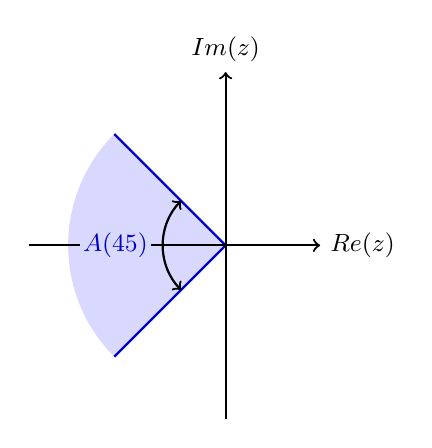
\begin{tikzpicture}

    % Parametri scalati per un grafico più piccolo
    \def\theta{45} % Ampiezza dell'angolo
    \def\R{2}      % Raggio della regione dimezzato

    % Colora la regione A(theta)
    \fill[blue!15] (0,0) -- ({180-\theta}:\R) arc ({180-\theta}:{180+\theta}:\R) -- cycle;

    % Disegna i bordi del cono
    \draw[thick, blue!80!black] (0,0) -- ({180-\theta}:\R);
    \draw[thick, blue!80!black] (0,0) -- ({180+\theta}:\R);

    % Disegna gli assi (molto più corti)
    \draw[->, thick] (-2.5, 0) -- (1.2, 0) node[right, font=\small] {$\operatorname{Re}(z)$};
    \draw[->, thick] (0, -2.2) -- (0, 2.2) node[above, font=\small] {$\operatorname{Im}(z)$};

    % Disegna gli archi per indicare l'angolo \theta (raggio ridotto)
    \draw[->, thick] (-0.8, 0) arc (180:{180-\theta}:0.8) node[midway, left=2pt, above=-1pt, font=\small] {};
    \draw[->, thick] (-0.8, 0) arc (180:{180+\theta}:0.8) node[midway, left=2pt, below=-1pt, font=\small] {};

    % Etichetta per la regione
    \node[blue!80!black] at (-1.4, 0) [fill=blue!15, inner sep=1pt, font=\small] {$A(\theta)$};

\end{tikzpicture}\\
Prendiamo in esempio l'equazione del calore
\[
\begin{cases}
	u_t = u_{xx} \ \ [0,1]\times\R^+\\
	u(x,0) = u_0(x)
\end{cases}
.\] 
$x_i = i\Delta x$ \ \  $u_{xx}(x_i)\approx \frac{u(x_{i+1}) - 2u(x_i) + u(x_{i-1})}{\Delta x^2}$  \ \ \ $O(\Delta x^2)$
 \[
	 u_t(x_i) = \frac{u(x_{i+1} - 2u(x_i) + u(x_{i-1})}{\Delta x^2} \ \ i=-,\ldots, Nx
.\] 
Eulero in tempo
\[
	\frac{u^{n+1}(x_i) - u^n(x_i)}{\Delta t} = frazione precedente
.\] 
e questo è stabile se $\frac {\Delta t}{\Delta x^2}\leq \frac 12$\\
Questo per dire che possiamo riciclare quello che sappiamo per le ODE con le PDE.

\newpage
\end{document}
